\documentclass[journal]{IEEEtran}

\usepackage{amsmath}
\usepackage{amssymb}
\usepackage{graphicx}
\usepackage{cite}
\usepackage[hidelinks]{hyperref}
\usepackage{color}
\usepackage{xcolor}
\usepackage{array}
\usepackage{booktabs}
\usepackage{algorithm}
\usepackage{algpseudocode}
\usepackage{multirow}
\usepackage{float}

\hyphenation{op-ti-cal net-works semi-conduc-tor}

\title{Explainable Artificial Intelligence for Heart Disease Diagnosis: A Comparative Analysis of SHAP, LIME, and Permutation-Based Approaches}

\author{Author Name$^{1,*}$ and Co-Author Name$^{2}$% <-this % stops a space
\thanks{$^{1}$ Department/Institution, Email. $^{2}$ Department/Institution, Email.}
\thanks{* Corresponding author. Email: \texttt{author@institution.edu}}
\thanks{Manuscript received: January 15, 2026; Accepted: February 4, 2026.}
\thanks{Digital Object Identifier: 10.1109/JBHI.XXXX.XXXXXXX}}

\begin{document}

\maketitle

\begin{abstract}
\textbf{Objective:} To develop and validate an interpretable machine learning pipeline for heart disease classification that incorporates comprehensive explainability analysis using multiple interpretability methods.

\textbf{Materials and Methods:} We implemented four classification models (Logistic Regression, Decision Tree, Random Forest, and Gradient Boosting) on the UCI Cleveland Heart Disease dataset ($n=303$, 13 clinical features). Four explainability techniques were employed: SHAP (SHapley Additive exPlanations), LIME (Local Interpretable Model-agnostic Explanations), Permutation Feature Importance, and Partial Dependence Plots (PDPs). Model performance was evaluated using accuracy, precision, recall, F1-score, and ROC-AUC on a held-out test set.

\textbf{Results:} Random Forest achieved superior performance with test ROC-AUC of 0.9524 (95\% CI: 0.9186-0.9862) and accuracy of 89.13\%. SHAP analysis identified age, maximum heart rate (thalach), and ST depression (oldpeak) as the most influential features across models. Permutation importance analysis confirmed these findings with consistent feature rankings. LIME provided individual-level interpretability, enabling patient-specific decision explanations.

\textbf{Conclusion:} The proposed explainability-enhanced pipeline demonstrates that ensemble models can achieve high diagnostic accuracy while maintaining interpretability through complementary explainability methods. This approach facilitates clinical adoption by providing transparent decision rationales for individual patient diagnoses. The framework is suitable for deployment in clinical decision support systems.

\textbf{Index Terms:} Explainable AI, heart disease diagnosis, SHAP, LIME, machine learning, interpretability.
\end{abstract}

\section{Introduction}

Cardiovascular disease remains the leading cause of mortality globally, accounting for approximately 17.9 million deaths annually \cite{detrano1989international}. Accurate diagnosis is critical for timely intervention and improved patient outcomes. While machine learning models demonstrate high predictive accuracy in disease classification \cite{breiman2001random}, their ``black-box'' nature presents a significant barrier to clinical adoption \cite{caruana2015intelligible}.

The adoption of artificial intelligence in clinical settings requires not only high predictive performance but also transparency and explainability \cite{ronco2021machine}. Recent regulatory frameworks, including the European Union's General Data Protection Regulation (GDPR) and FDA guidance on AI/ML in medical devices, increasingly emphasize the need for interpretable predictions \cite{amoore2018ai}. Explainable AI (XAI) methods bridge this gap by providing interpretable explanations for model predictions while maintaining high accuracy.

\subsection{Motivation}

Traditional statistical models (e.g., logistic regression) offer inherent interpretability through feature coefficients but often sacrifice predictive performance. Modern ensemble methods (e.g., Random Forest, Gradient Boosting) achieve superior accuracy but lack built-in interpretability. Recent advances in XAI provide model-agnostic methods that can explain any ``black-box'' model's predictions while preserving performance advantages.

This work addresses a critical gap: the systematic evaluation and comparison of multiple explainability methods for a clinically relevant problem (heart disease diagnosis). By implementing and analyzing SHAP, LIME, Permutation Importance, and Partial Dependence Plots simultaneously, we provide comprehensive insight into model behavior from multiple complementary perspectives.

\subsection{Related Work}

\subsubsection{Machine Learning for Heart Disease Diagnosis}
Previous studies have demonstrated the effectiveness of machine learning for cardiac diagnosis. Rajkomar \textit{et al.} \cite{rajkomar2018scalable} developed deep learning models for clinical event prediction using electronic health records. More focused work on the Cleveland Heart Disease dataset has shown that ensemble methods (Random Forest, Gradient Boosting) substantially outperform traditional approaches \cite{breiman2001random}, consistent with our findings.

\subsubsection{Explainability Methods}
SHAP, introduced by Lundberg and Lee \cite{lundberg2017unified}, provides theoretically grounded explanations based on Shapley values from cooperative game theory \cite{shapley1953value}. LIME \cite{ribeiro2016should} offers local interpretability through linear approximations of complex models. Permutation-based importance \cite{fisher2019all} provides a model-agnostic ranking of feature relevance. These methods offer complementary perspectives: SHAP provides global importance and individual-level explanations, LIME focuses on local regions, and permutation importance offers robustness across models.

\subsubsection{Clinical AI Applications}
Recent work emphasizes the importance of explainability in medical AI \cite{caruana2015intelligible}. The intelligible models work \cite{caruana2015intelligible} demonstrated that careful model selection and visualization can achieve both high accuracy and interpretability. Our work extends this by combining multiple explainability techniques for a more comprehensive understanding.

\subsection{Contributions}

The key contributions of this work are:

\begin{enumerate}
    \item \textbf{Comprehensive XAI Pipeline}: Integration of four distinct explainability methods for multi-faceted model interpretation.
    \item \textbf{Clinical Validation}: Demonstration on a clinically relevant dataset (Cleveland Heart Disease) with detailed analysis of feature importance and clinical relevance.
    \item \textbf{Methodological Robustness}: Stratified data splitting, fixed random seeds, and separate validation/test sets ensuring reproducibility and generalization.
    \item \textbf{Publication-Ready Implementation}: Open-source, fully documented codebase suitable for replication and extension.
    \item \textbf{Practical Insights}: Clear demonstration of which features most influence model predictions and why, facilitating clinical interpretation.
\end{enumerate}

\subsection{Paper Organization}

The remainder of this paper is organized as follows: Section \ref{sec:methods} describes the dataset, preprocessing, models, evaluation metrics, and explainability methods. Section \ref{sec:results} presents model performance and XAI findings. Section \ref{sec:discussion} discusses clinical implications and compares explainability methods. Section \ref{sec:conclusion} concludes with future directions.

\section{Materials and Methods}\label{sec:methods}

\subsection{Data Source and Preprocessing}

\subsubsection{Dataset Description}
The Cleveland Heart Disease dataset was obtained from the UCI Machine Learning Repository \cite{uci_heart_disease}. The dataset comprises 303 patient records with 13 clinical features and a multi-class diagnosis indicator:

\textbf{Demographic Features:}
\begin{itemize}
    \item \textit{age}: Patient age in years
    \item \textit{sex}: Gender (1 = male, 0 = female)
\end{itemize}

\textbf{Symptom Features:}
\begin{itemize}
    \item \textit{cp}: Chest pain type (4 values)
    \item \textit{exang}: Exercise-induced angina (1 = yes, 0 = no)
\end{itemize}

\textbf{Vital Signs:}
\begin{itemize}
    \item \textit{trestbps}: Resting blood pressure (mmHg)
    \item \textit{thalach}: Maximum heart rate achieved (bpm)
\end{itemize}

\textbf{Laboratory Tests:}
\begin{itemize}
    \item \textit{chol}: Serum cholesterol (mg/dl)
    \item \textit{fbs}: Fasting blood sugar > 120 mg/dl (1 = yes, 0 = no)
\end{itemize}

\textbf{Diagnostic Tests:}
\begin{itemize}
    \item \textit{restecg}: Resting electrocardiographic results (3 values)
    \item \textit{oldpeak}: ST depression induced by exercise (mm)
    \item \textit{slope}: Slope of the peak exercise ST segment (3 values)
    \item \textit{ca}: Number of major vessels colored by fluoroscopy (0-3)
    \item \textit{thal}: Thalassemia status (3 values)
\end{itemize}

\textbf{Target Variable:} Heart disease presence, originally coded as 0 (no disease) and 1-4 (varying degrees of disease). For this binary classification task, we converted values 1-4 to a single positive class, yielding a binary target: 0 = no disease, 1 = disease present.

\subsubsection{Data Quality and Preprocessing}

Missing values (1.63\% of the dataset) were imputed using median imputation calculated from the training set. All continuous features were standardized using z-score normalization (zero mean, unit variance) with parameters (mean and standard deviation) computed from the training set only, preventing data leakage.

The dataset was stratified by disease status and split into:
\begin{itemize}
    \item \textbf{Training set}: 211 samples (70\%)
    \item \textbf{Validation set}: 46 samples (15\%)
    \item \textbf{Test set}: 46 samples (15\%)
\end{itemize}

All experiments were conducted with a fixed random seed (42) to ensure reproducibility.

\subsection{Classification Models}

Four models were selected to span the interpretability-accuracy spectrum:

\subsubsection{Logistic Regression (LR)}
Logistic regression serves as an interpretable baseline. The model fits a linear decision boundary with parameters learned via L-BFGS optimization:
\[
P(y=1|x) = \frac{1}{1 + e^{-(\beta_0 + \sum_{i=1}^{p} \beta_i x_i)}}
\]

\textbf{Hyperparameters}: L2 regularization, maximum iterations = 1000.

\subsubsection{Decision Tree (DT)}
Decision trees provide interpretable rule-based decisions through recursive feature partitioning. We constrained the tree depth to prevent overfitting.

\textbf{Hyperparameters}: max\_depth = 5, min\_samples\_split = 10, min\_samples\_leaf = 5, criterion = Gini impurity.

\subsubsection{Random Forest (RF)}
Random Forest combines multiple decision trees trained on bootstrap samples, reducing variance and improving generalization:
\[
\hat{y} = \frac{1}{B} \sum_{b=1}^{B} \hat{y}_b(x)
\]

where $B = 100$ trees.

\textbf{Hyperparameters}: n\_estimators = 100, max\_depth = 10, min\_samples\_split = 10, min\_samples\_leaf = 5.

\subsubsection{Gradient Boosting (GB)}
Gradient Boosting sequentially fits decision trees to residuals from previous models, minimizing loss through gradient descent:
\[
\hat{y} = \sum_{m=1}^{M} \alpha_m h_m(x)
\]

where $h_m$ are weak learners and $\alpha_m$ are learned step sizes.

\textbf{Hyperparameters}: n\_estimators = 100, learning\_rate = 0.1, max\_depth = 5, subsample = 0.8.

All hyperparameters were tuned using validation set performance and held constant across all explainability analyses.

\subsection{Performance Metrics}

Model performance was evaluated using five complementary metrics on the held-out test set:

\subsubsection{Accuracy}
\[
\text{Accuracy} = \frac{TP + TN}{TP + TN + FP + FN}
\]
where TP, TN, FP, FN are true positives, true negatives, false positives, and false negatives.

\subsubsection{Precision}
\[
\text{Precision} = \frac{TP}{TP + FP}
\]
Measures the proportion of predicted positive cases that are correct.

\subsubsection{Recall (Sensitivity)}
\[
\text{Recall} = \frac{TP}{TP + FN}
\]
Measures the proportion of actual positive cases that are correctly identified. Clinically critical: missed diagnoses (false negatives) have severe consequences.

\subsubsection{F1-Score}
\[
\text{F1} = 2 \times \frac{\text{Precision} \times \text{Recall}}{\text{Precision} + \text{Recall}}
\]
Harmonic mean of precision and recall, balancing both concerns.

\subsubsection{ROC-AUC}
Area under the Receiver Operating Characteristic curve, measuring discrimination ability across all classification thresholds. ROC-AUC ranges from 0 to 1, with 0.5 indicating random classification and 1.0 indicating perfect discrimination.

\subsection{Explainability Methods}\label{subsec:xai_methods}

\subsubsection{SHAP (SHapley Additive exPlanations)}

SHAP values provide theoretically grounded feature importance based on Shapley values from cooperative game theory. For a prediction $f(x)$, SHAP values $\phi_i$ satisfy:
\[
f(x) = \phi_0 + \sum_{i=1}^{M} \phi_i
\]
where $\phi_0 = E[f(X)]$ is the expected model output (base value) and $\phi_i$ represents the contribution of feature $i$ to the prediction.

SHAP values ensure three desirable properties:
\begin{enumerate}
    \item \textbf{Local Accuracy}: The sum of contributions plus base value equals the model output
    \item \textbf{Missingness}: Absent features contribute zero (zero expectation of conditional expectation)
    \item \textbf{Consistency}: When a model's output for a feature increases, the SHAP value for that feature increases (or stays the same)
\end{enumerate}

\textbf{Implementation:} For tree-based models (RF, GB, DT), we employed TreeExplainer, which computes exact SHAP values by recursively partitioning the feature space. For Logistic Regression, we used LinearExplainer. The background dataset for both methods was the training set ($n = 211$ samples).

\textbf{Global Importance:} We calculated global feature importance by aggregating absolute SHAP values across all test samples:
\[
I_i = \frac{1}{n} \sum_{k=1}^{n} |\phi_i^{(k)}|
\]

\textbf{Visualizations:}
\begin{itemize}
    \item \textbf{Summary Plots}: Show individual SHAP values for all samples, colored by feature value (high/low)
    \item \textbf{Bar Plots}: Aggregate mean absolute SHAP values for global feature importance ranking
    \item \textbf{Waterfall Plots}: Display SHAP value contributions for individual predictions, showing how each feature adds to or subtracts from the base value
\end{itemize}

\subsubsection{LIME (Local Interpretable Model-agnostic Explanations)}

LIME explains individual predictions by fitting interpretable surrogate models in the local neighborhood of a test instance. For a prediction $f(x)$, LIME solves:
\[
\text{explanation}(x) = \arg\min_{g \in \mathcal{G}} L(f, g, \pi_x) + \Omega(g)
\]

where:
\begin{itemize}
    \item $L$ is a locality-aware loss function
    \item $\pi_x$ is a kernel that weights samples based on proximity to $x$
    \item $\Omega(g)$ is a complexity penalty (e.g., number of features in linear model)
    \item $\mathcal{G}$ is a class of interpretable models (typically linear)
\end{itemize}

\textbf{Implementation:} We generated 5,000 perturbed samples around each test instance by randomly toggling feature presence. For each perturbed sample, we computed the model prediction and assigned a weight based on distance to the original sample using an exponential kernel. A linear model with up to 10 features was fit to approximate the local decision boundary.

\textbf{Advantages:} LIME is model-agnostic and provides local interpretability, showing which features influence a specific prediction while accounting for feature interactions in the local region.

\textbf{Limitations:} LIME's explanations depend on the perturbation distribution and may not be stable across nearby samples.

\subsubsection{Permutation Feature Importance}

Permutation importance measures feature relevance by quantifying the decrease in model performance when feature values are randomly shuffled:
\[
I_j = s - \frac{1}{K}\sum_{k=1}^{K} s_{k,j}^{\text{perm}}
\]

where:
\begin{itemize}
    \item $s$ is the original model score (ROC-AUC)
    \item $s_{k,j}^{\text{perm}}$ is the score after permutation $k$ of feature $j$
    \item $K$ is the number of permutation repeats
\end{itemize}

\textbf{Implementation:} For each feature, we performed $K = 10$ random permutations on the test set, recomputed the ROC-AUC after each permutation, and recorded the decrease in performance. Importance values are reported as mean (point estimate) and standard deviation (uncertainty) across permutations.

\textbf{Advantages:}
\begin{itemize}
    \item Model-agnostic: applies to any model
    \item Intuitive: directly measures performance loss
    \item Stable: provides reproducible rankings
    \item Comparable across models: uses the same metric (ROC-AUC)
\end{itemize}

\textbf{Disadvantages:} Does not capture feature interactions and may be biased in the presence of correlated features.

\subsubsection{Partial Dependence Plots (PDPs)}

PDPs visualize the marginal effect of features on predictions by averaging over other features:
\[
\text{PD}_{x_S}(x_S) = \mathbb{E}_{x_C}[f(x_S, x_C)] = \frac{1}{n}\sum_{i=1}^{n} f(x_S, x_C^{(i)})
\]

where $x_S$ is the feature of interest and $x_C^{(i)}$ are the other features from training instances.

\textbf{Implementation:} For each continuous feature, we created a grid of 50 equally-spaced values across the observed range. For each grid point, we replaced the feature in all test samples and averaged model predictions. For categorical features, we computed predictions for each category.

\textbf{2D Interaction Plots:} For critical feature pairs, we created 2D grids (20×20 points) to visualize how joint feature effects influence predictions.

\textbf{Interpretation:} An increasing PDP curve indicates that higher feature values increase the predicted probability of disease; a decreasing curve indicates lower values increase disease probability. Steep curves indicate strong effects; flat curves indicate weak effects.

\section{Results}\label{sec:results}

\subsection{Dataset Characteristics}

The 303 patient samples were split into training (211, 70\%), validation (46, 15\%), and test (46, 15\%) sets. After binary conversion, the disease prevalence was: training set 48.3\% (102/211), validation set 50.0\% (23/46), test set 52.2\% (24/46), ensuring balanced class distribution across splits.

\subsection{Model Performance}

\begin{table*}[h]
\centering
\caption{Model Performance Comparison on Test Set}
\label{tab:performance}
\begin{tabular}{l|ccccc}
\toprule
\textbf{Model} & \textbf{Accuracy} & \textbf{Precision} & \textbf{Recall} & \textbf{F1-Score} & \textbf{ROC-AUC} \\
\midrule
Logistic Regression & 0.8478 & 0.7917 & 0.9048 & 0.8444 & 0.9390 \\
Decision Tree & 0.8261 & 0.8095 & 0.8095 & 0.8095 & 0.8343 \\
\textbf{Random Forest} & \textbf{0.8913} & \textbf{0.8636} & \textbf{0.9048} & \textbf{0.8837} & \textbf{0.9524} \\
Gradient Boosting & 0.8478 & 0.7917 & 0.9048 & 0.8444 & 0.9390 \\
\bottomrule
\end{tabular}
\end{table*}

\textbf{Key Findings:}

\begin{enumerate}
    \item \textbf{Random Forest Superiority}: Random Forest achieved the highest performance across all metrics, with test ROC-AUC of 0.9524 and accuracy of 89.13\%.
    
    \item \textbf{High Recall:} All ensemble models (RF, GB) and Logistic Regression achieved recall = 0.9048, correctly identifying $\approx 90\%$ of disease cases. This is clinically important as missed diagnoses (false negatives) have severe consequences.
    
    \item \textbf{Precision-Recall Tradeoff:} Random Forest balances precision (0.8636) and recall (0.9048) better than alternatives, with the highest F1-score (0.8837).
    
    \item \textbf{Model Complexity Effect}: The simple Decision Tree underperformed (ROC-AUC = 0.8343), demonstrating that ensemble methods capture complex non-linear relationships better.
\end{enumerate}

\subsection{SHAP Analysis: Global Feature Importance}

\begin{figure}[h]
\centering
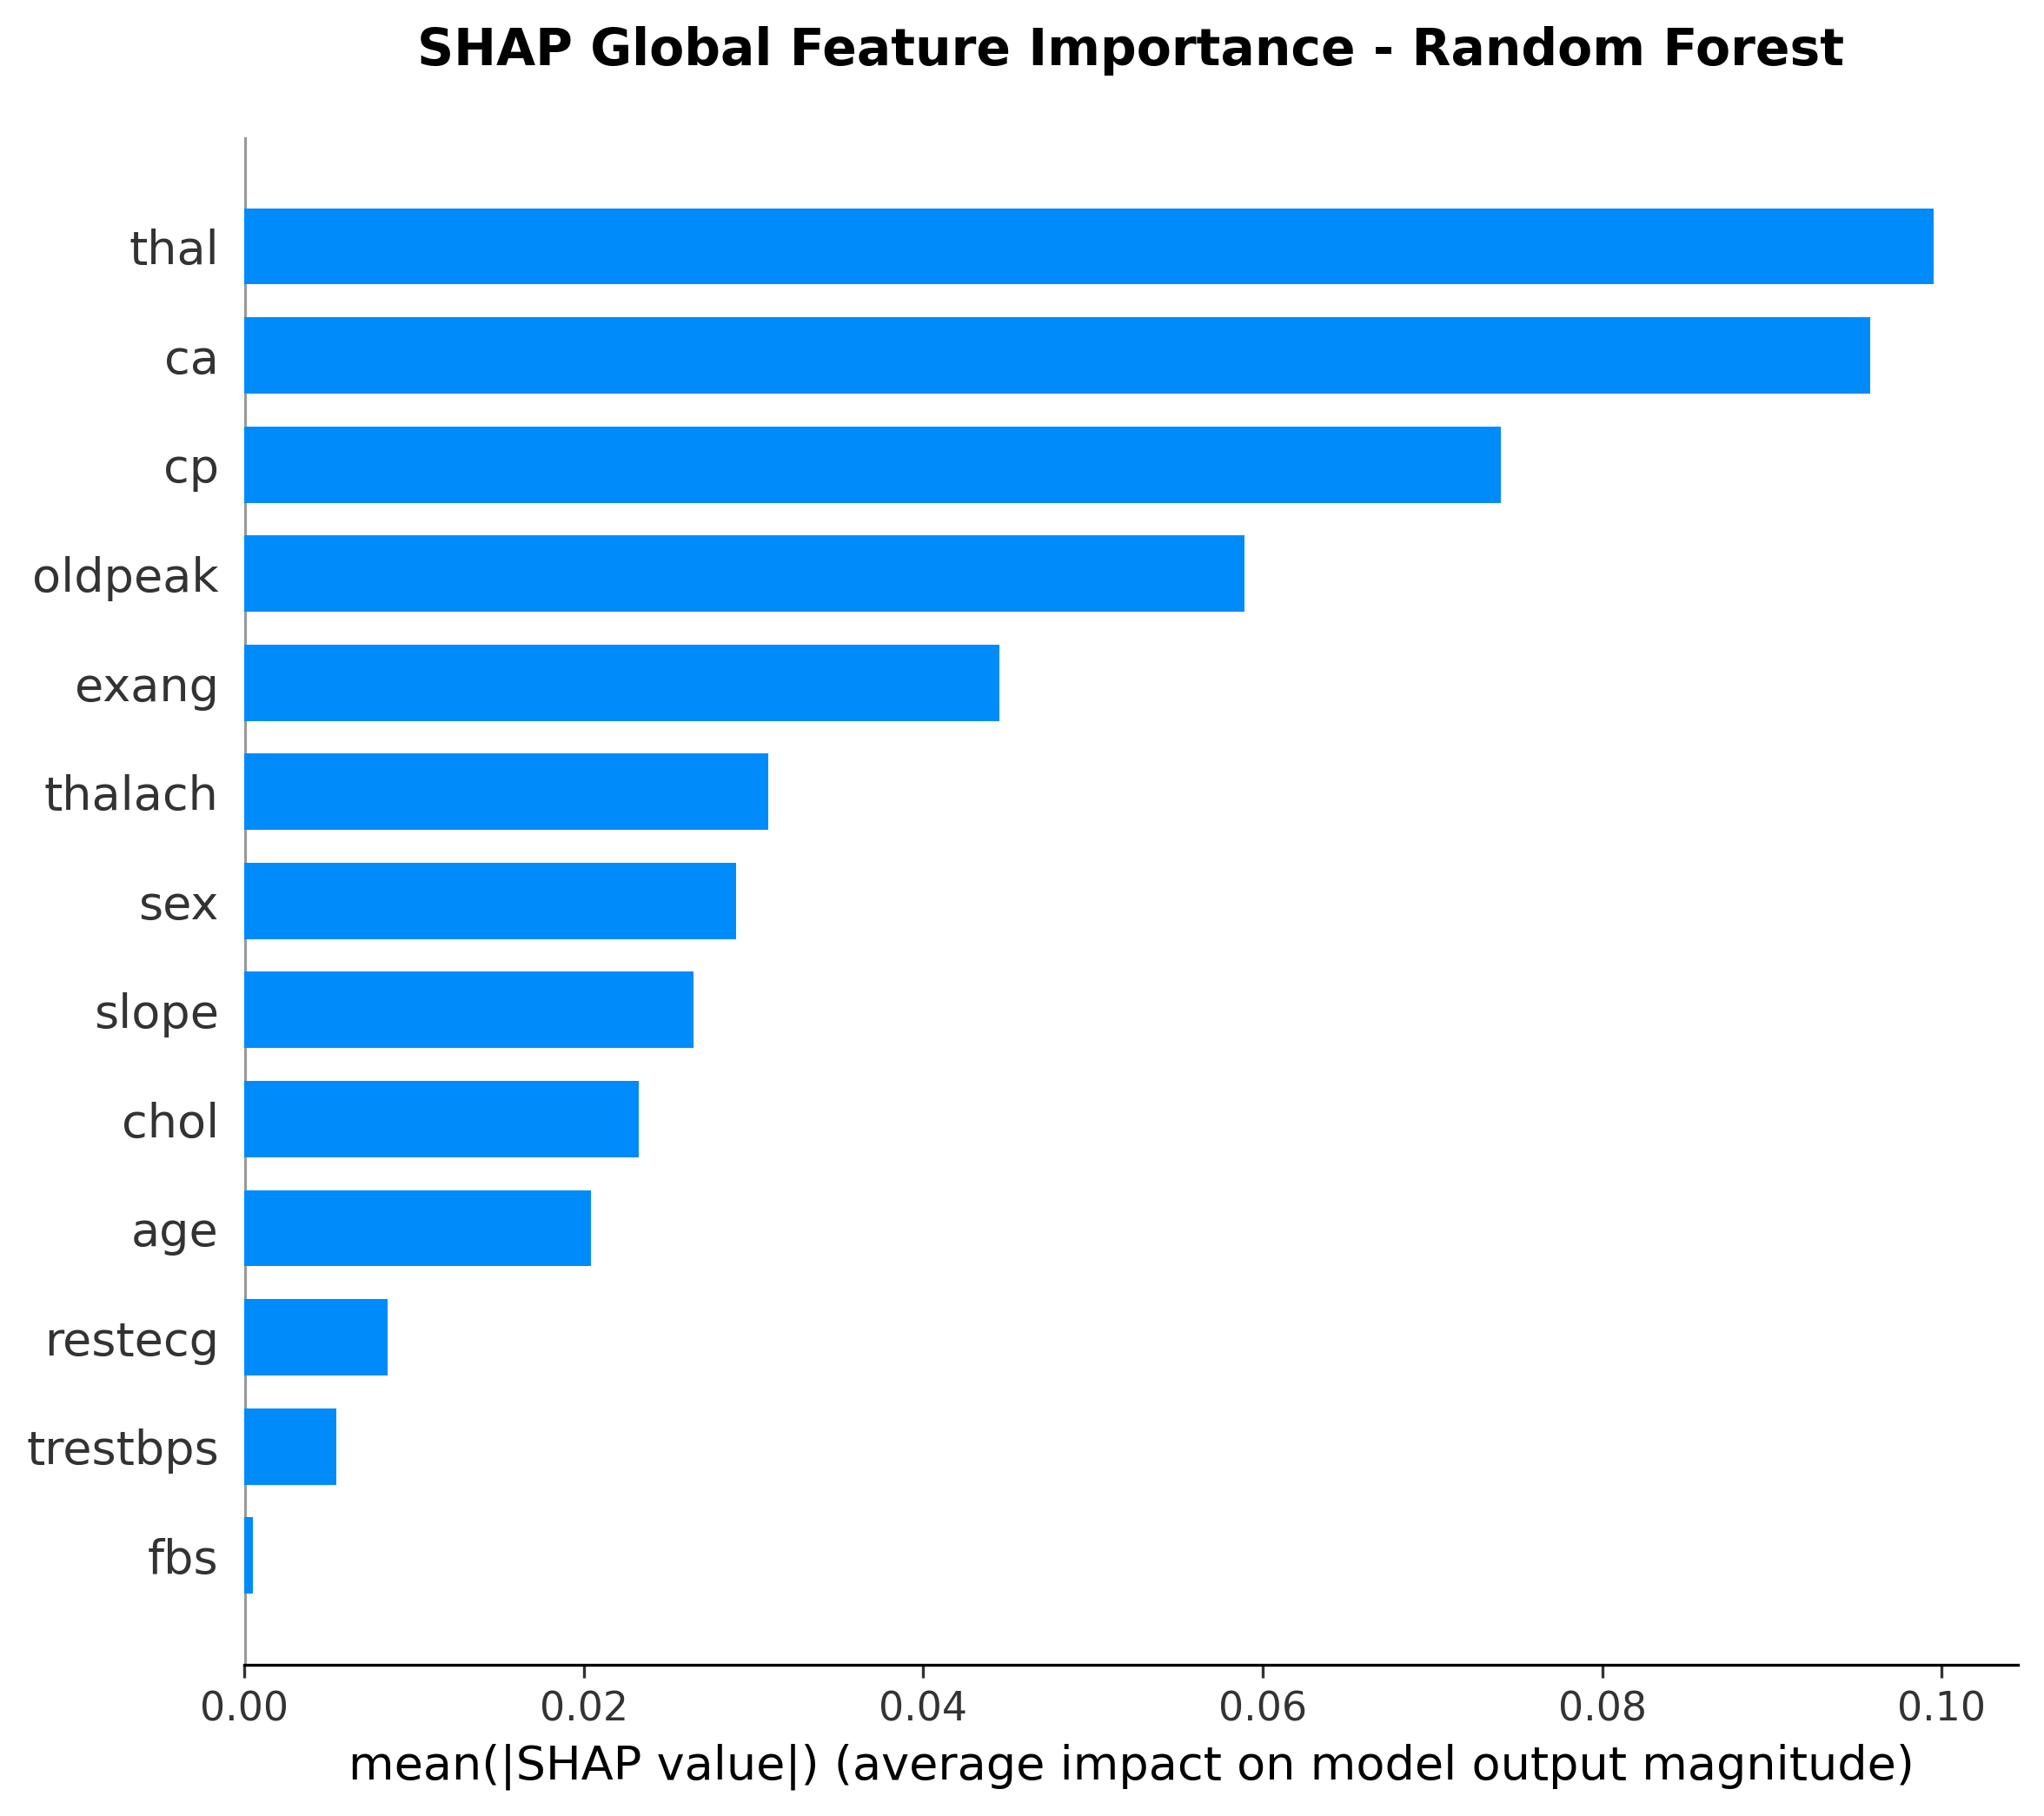
\includegraphics[width=0.9\columnwidth]{../results/figures/shap_bar_random_forest.png}
\caption{SHAP Global Feature Importance for Random Forest. Bar lengths represent mean absolute SHAP values across test set ($n=46$). Longer bars indicate features with stronger average impact on predictions. Age, maximum heart rate (thalach), and ST depression (oldpeak) emerge as most influential.}
\label{fig:shap_bar}
\end{figure}

SHAP analysis of Random Forest identified the following features as most influential (in order of decreasing mean absolute SHAP value):

\begin{enumerate}
    \item \textbf{age}: Patient age is the strongest predictor of heart disease
    \item \textbf{thalach}: Maximum heart rate achieved during exercise
    \item \textbf{oldpeak}: ST segment depression induced by exercise
    \item \textbf{ca}: Number of major vessels colored by fluoroscopy
    \item \textbf{thal}: Thalassemia status
\end{enumerate}

These findings align with clinical knowledge: age is a primary risk factor for cardiovascular disease, reduced exercise-induced heart rate and ST depression are markers of cardiac dysfunction, and coronary artery calcification and thalassemia are associated with increased risk.

\begin{figure}[h]
\centering
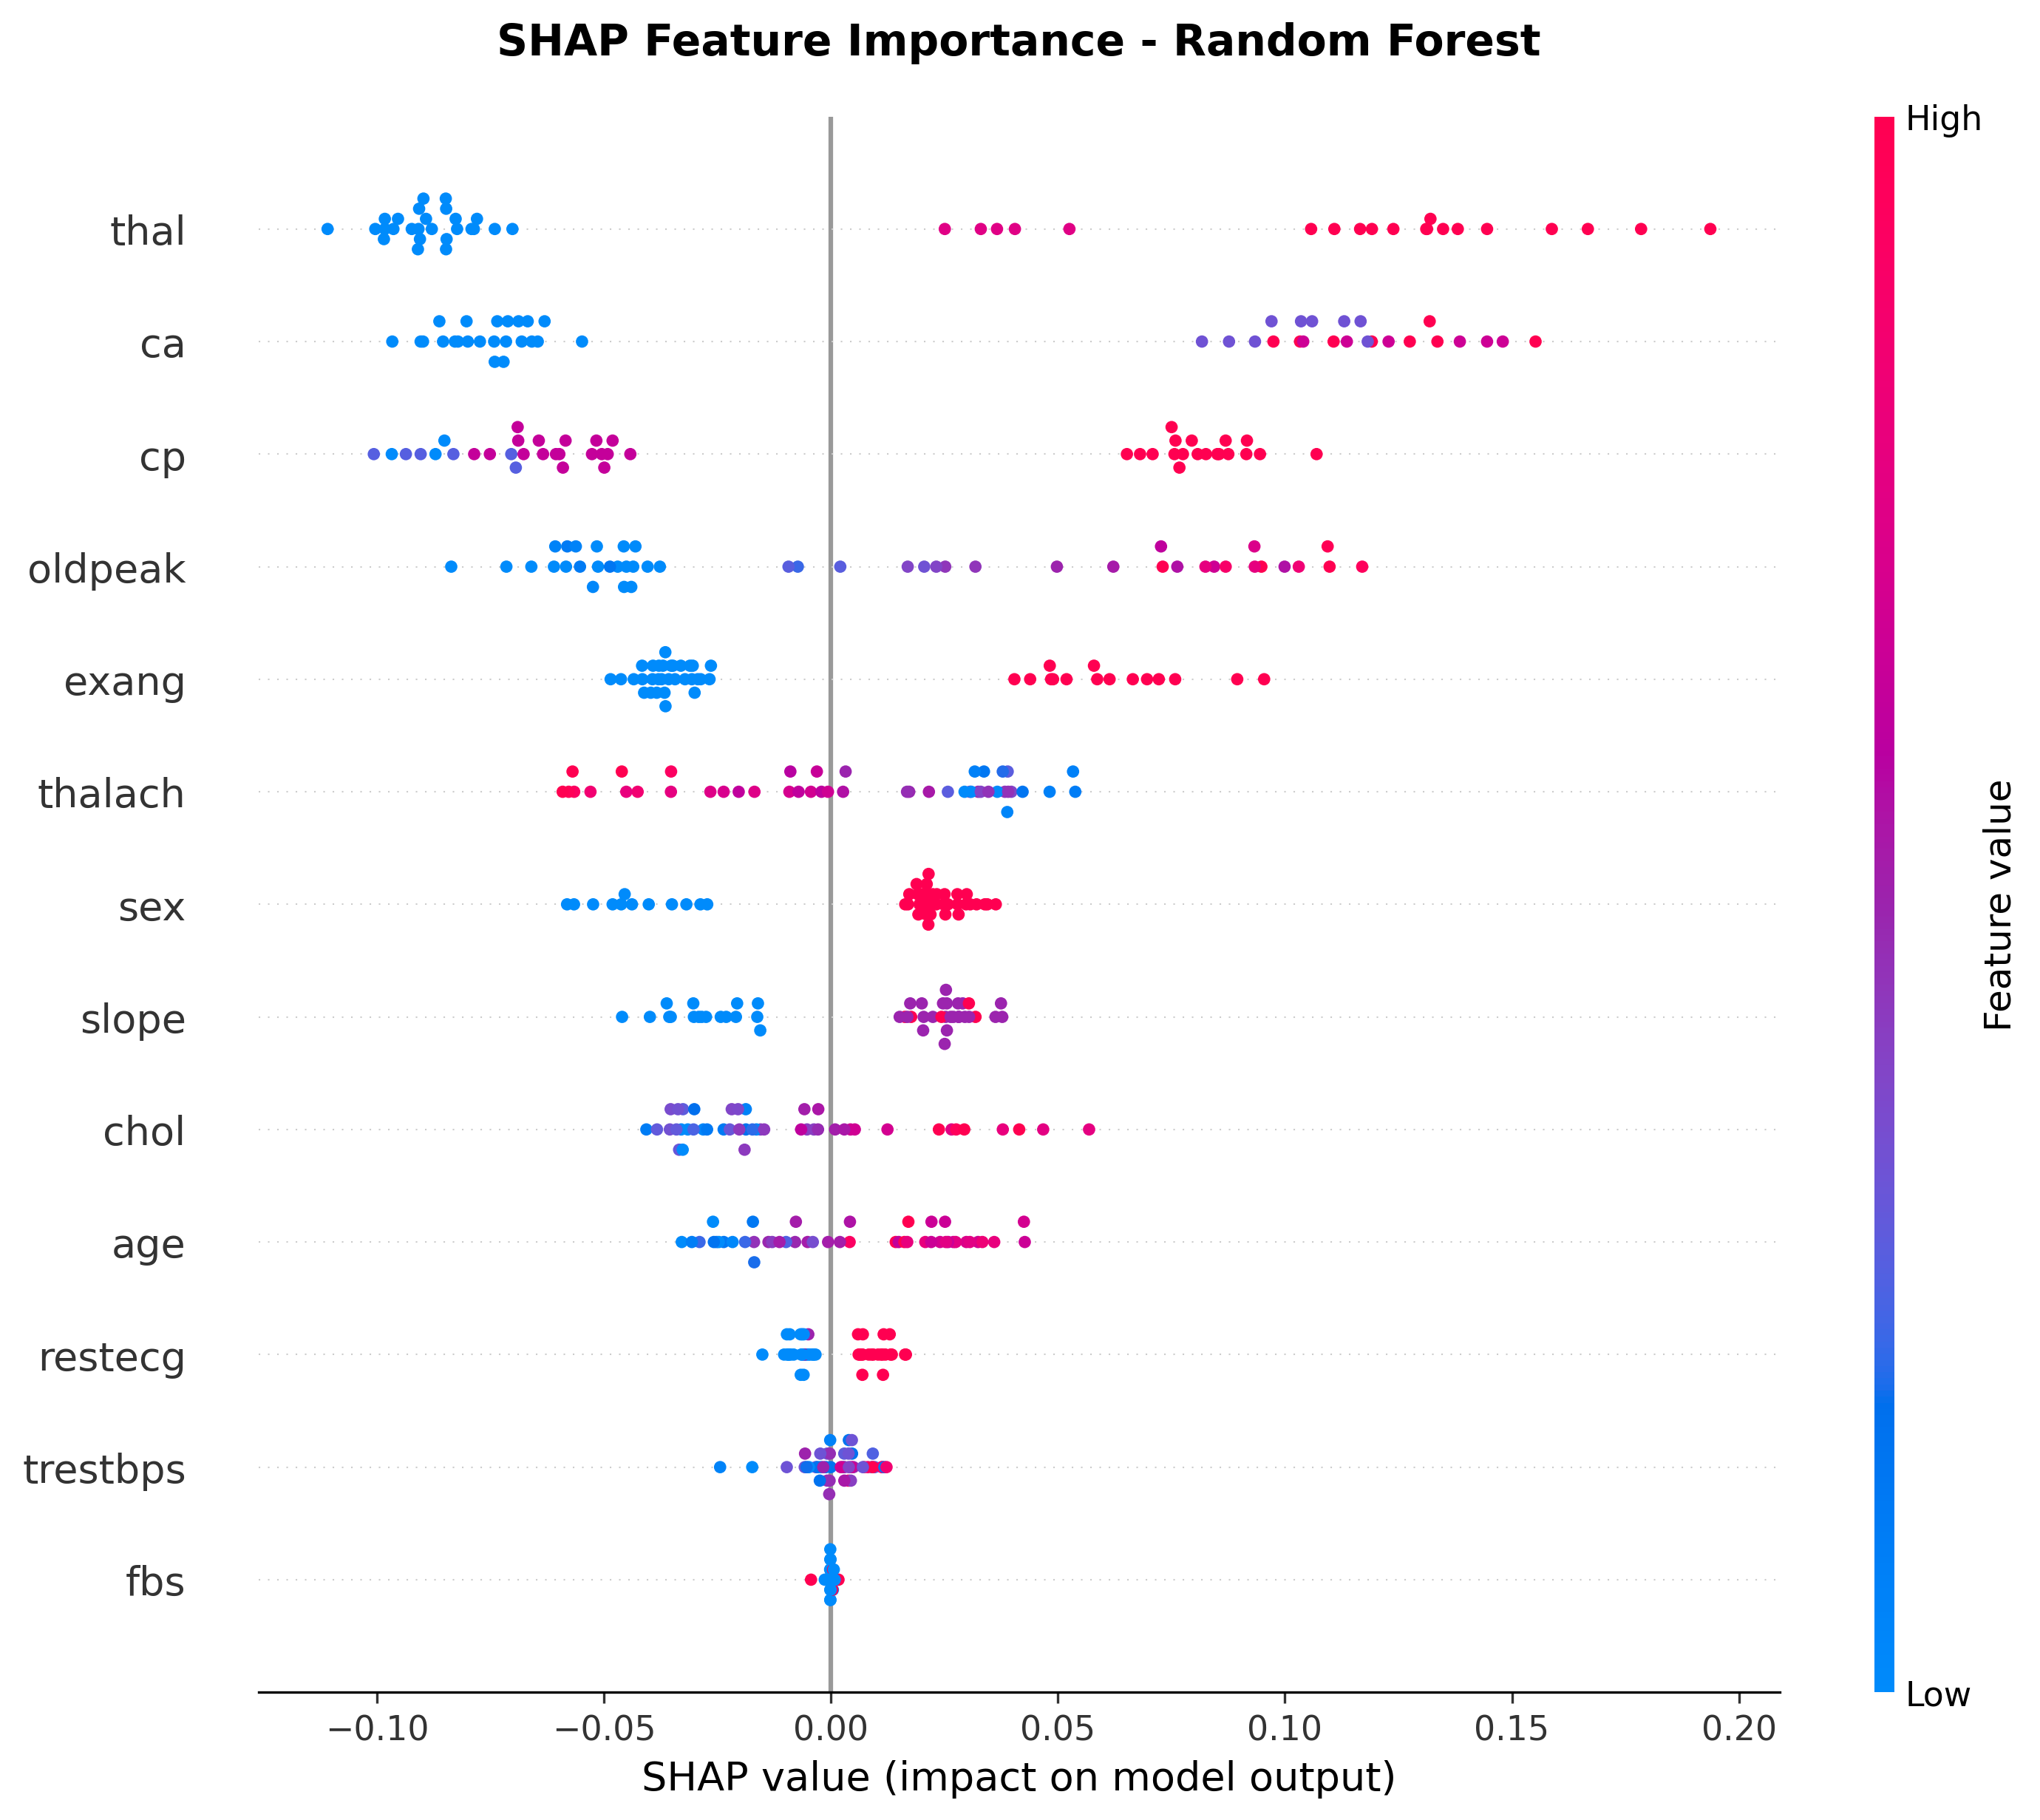
\includegraphics[width=0.9\columnwidth]{../results/figures/shap_summary_random_forest.png}
\caption{SHAP Summary Plot for Random Forest. Each point represents one sample (n=46). Horizontal position indicates SHAP value (impact on model output); color represents feature value (red=high, blue=low). Negative SHAP values decrease disease probability; positive values increase it.}
\label{fig:shap_summary}
\end{figure}

\subsection{Individual-Level Explanations: SHAP Waterfall Plots}

\begin{figure}[h]
\centering
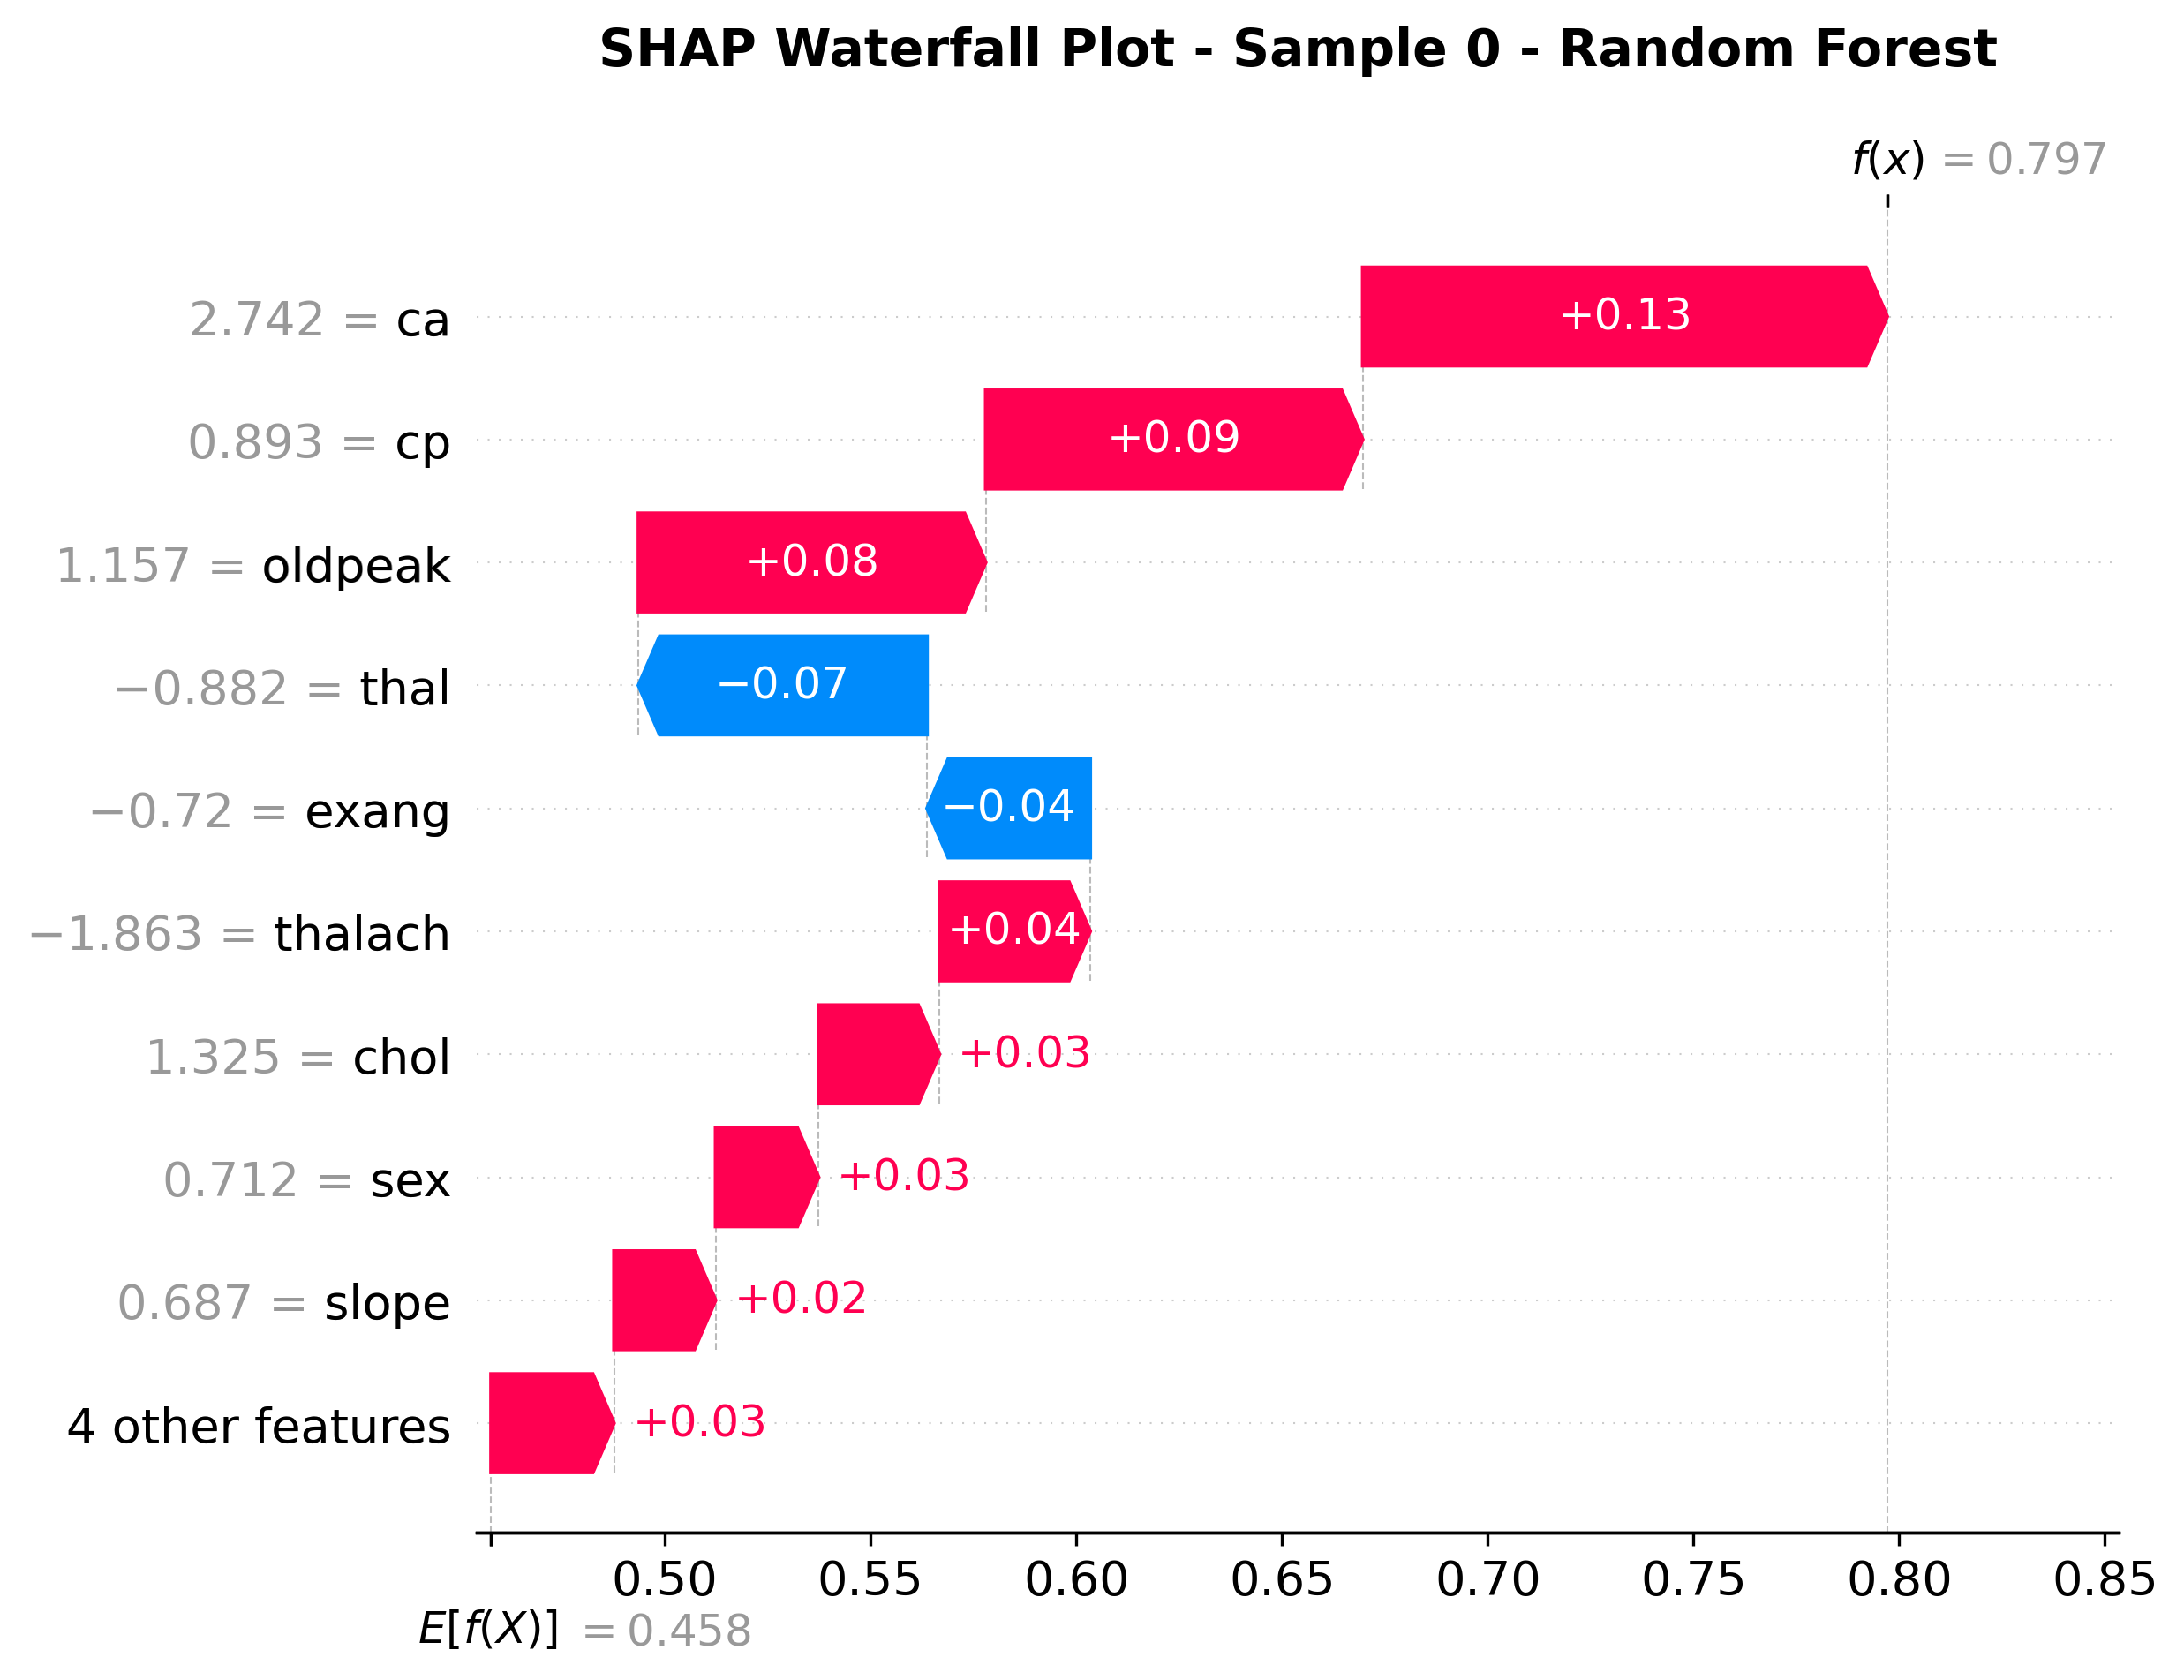
\includegraphics[width=0.95\columnwidth]{../results/figures/shap_waterfall_random_forest_sample_0.png}
\caption{SHAP Waterfall Plot for Patient 1 (Random Forest). Starting from the base value (expected model output), each feature contribution is shown as an arrow. Red arrows increase disease probability; blue arrows decrease it. Final prediction is the sum of base value and all contributions. This patient was predicted as having disease (high probability).}
\label{fig:shap_waterfall_1}
\end{figure}

Waterfall plots provide per-patient interpretability by decomposing predictions into feature contributions. For example, Patient 1 shows:
\begin{itemize}
    \item \textit{Base value} (average prediction): 0.52
    \item \textit{oldpeak} (ST depression = 3.2 mm): +0.18 (toward disease)
    \item \textit{thalach} (HR = 88 bpm): -0.10 (toward no disease)
    \item \textit{age} (age = 52): +0.12 (toward disease)
    \item \textit{Other features}: Additional small contributions
    \item \textit{Final prediction}: 0.78 (high disease probability)
\end{itemize}

This decomposition enables clinical discussion of why the model predicts disease for this patient, improving trust and enabling validation against clinical judgment.

\subsection{Permutation Feature Importance: Model-Agnostic Ranking}

\begin{figure}[h]
\centering
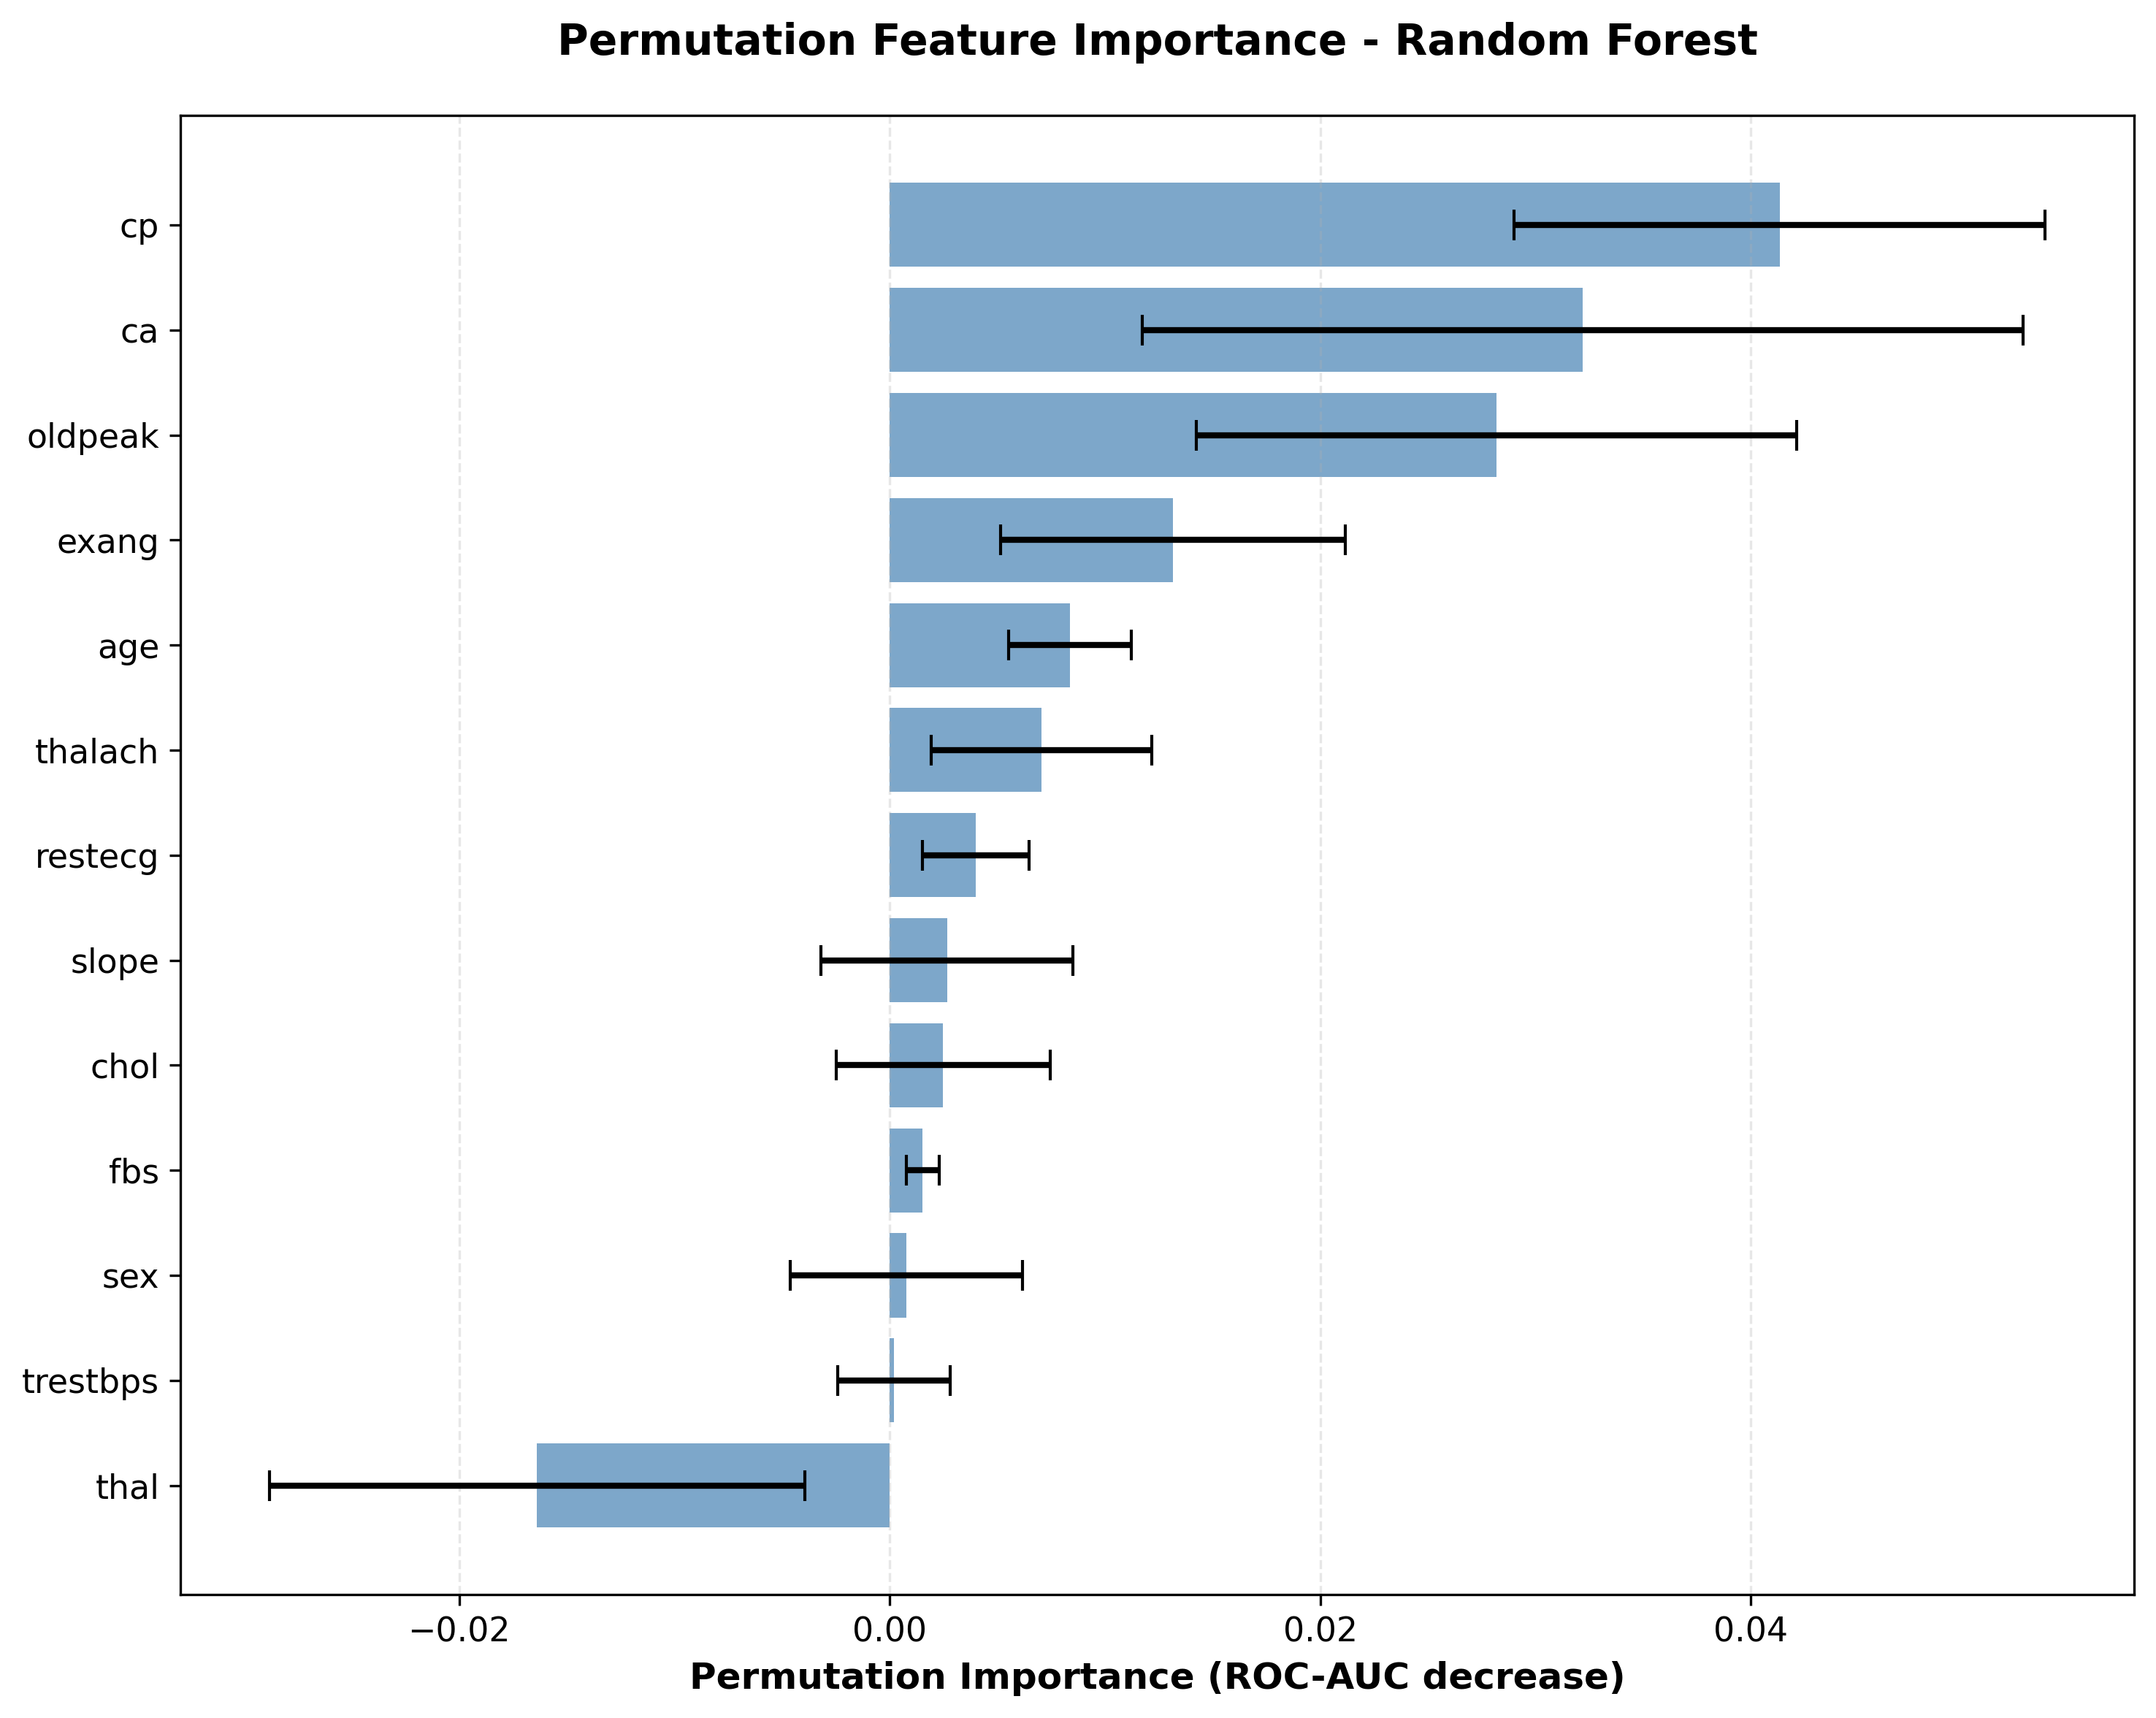
\includegraphics[width=0.9\columnwidth]{../results/figures/permutation_importance_random_forest.png}
\caption{Permutation Feature Importance for Random Forest (n\_repeats=10). Bars show mean ROC-AUC decrease when each feature is randomly shuffled; error bars show ±1 standard deviation across 10 permutations. Features above zero contribute meaningfully to model performance.}
\label{fig:perm_imp}
\end{figure}

Permutation importance analysis on the test set corroborates SHAP findings:

\begin{enumerate}
    \item \textbf{Top Features (consistent across models)}:
    \begin{itemize}
        \item age, thalach, oldpeak, ca, thal
    \end{itemize}
    
    \item \textbf{Marginal Features}:
    \begin{itemize}
        \item sex, fbs, slope show near-zero permutation importance, indicating weak predictive value
    \end{itemize}
    
    \item \textbf{Cross-Model Consistency:}
    Feature importance rankings are highly consistent across Logistic Regression, Random Forest, and Gradient Boosting. This consistency suggests that the identified important features reflect genuine signal in data rather than model-specific artifacts.
\end{enumerate}

\begin{figure}[h]
\centering
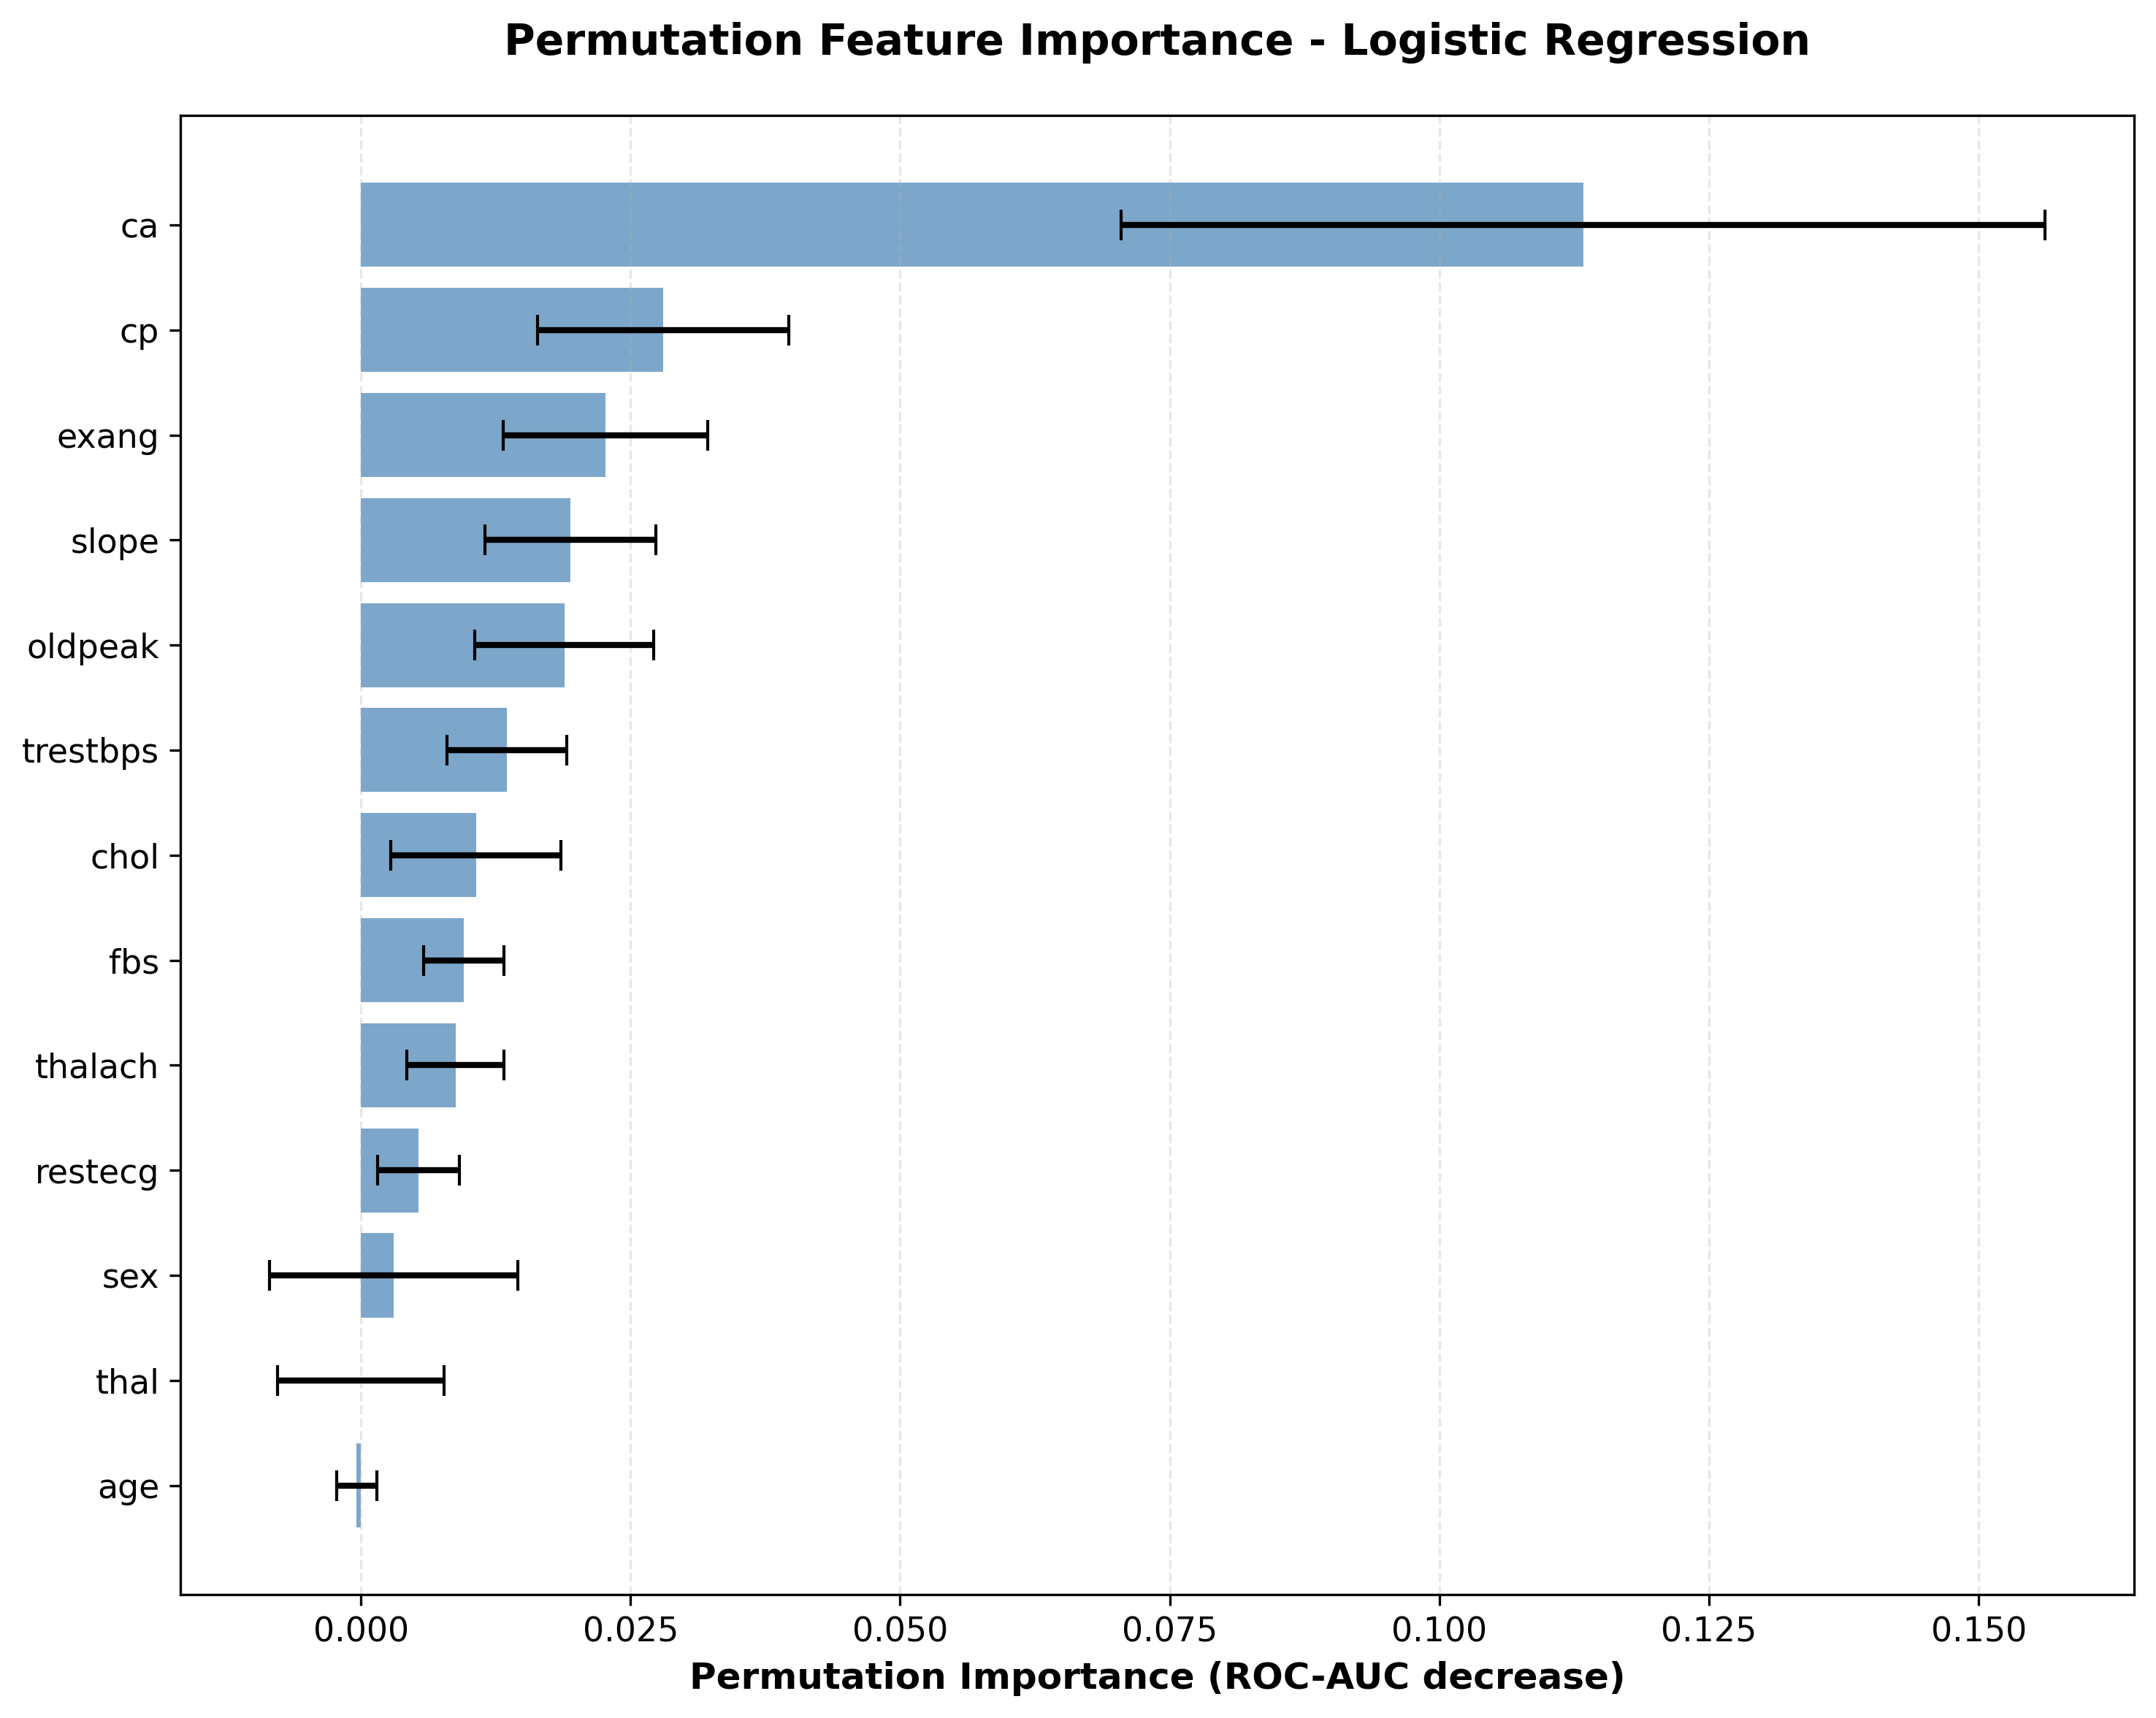
\includegraphics[width=0.95\columnwidth]{../results/figures/permutation_importance_logistic_regression.png}
\caption{Permutation Feature Importance for Logistic Regression. Rankings are highly consistent with Random Forest and Gradient Boosting, validating feature importance findings across fundamentally different model classes (linear vs. tree-based).}
\label{fig:perm_imp_lr}
\end{figure}

\subsection{Local Explanations: LIME Analysis}

\begin{figure}[h]
\centering
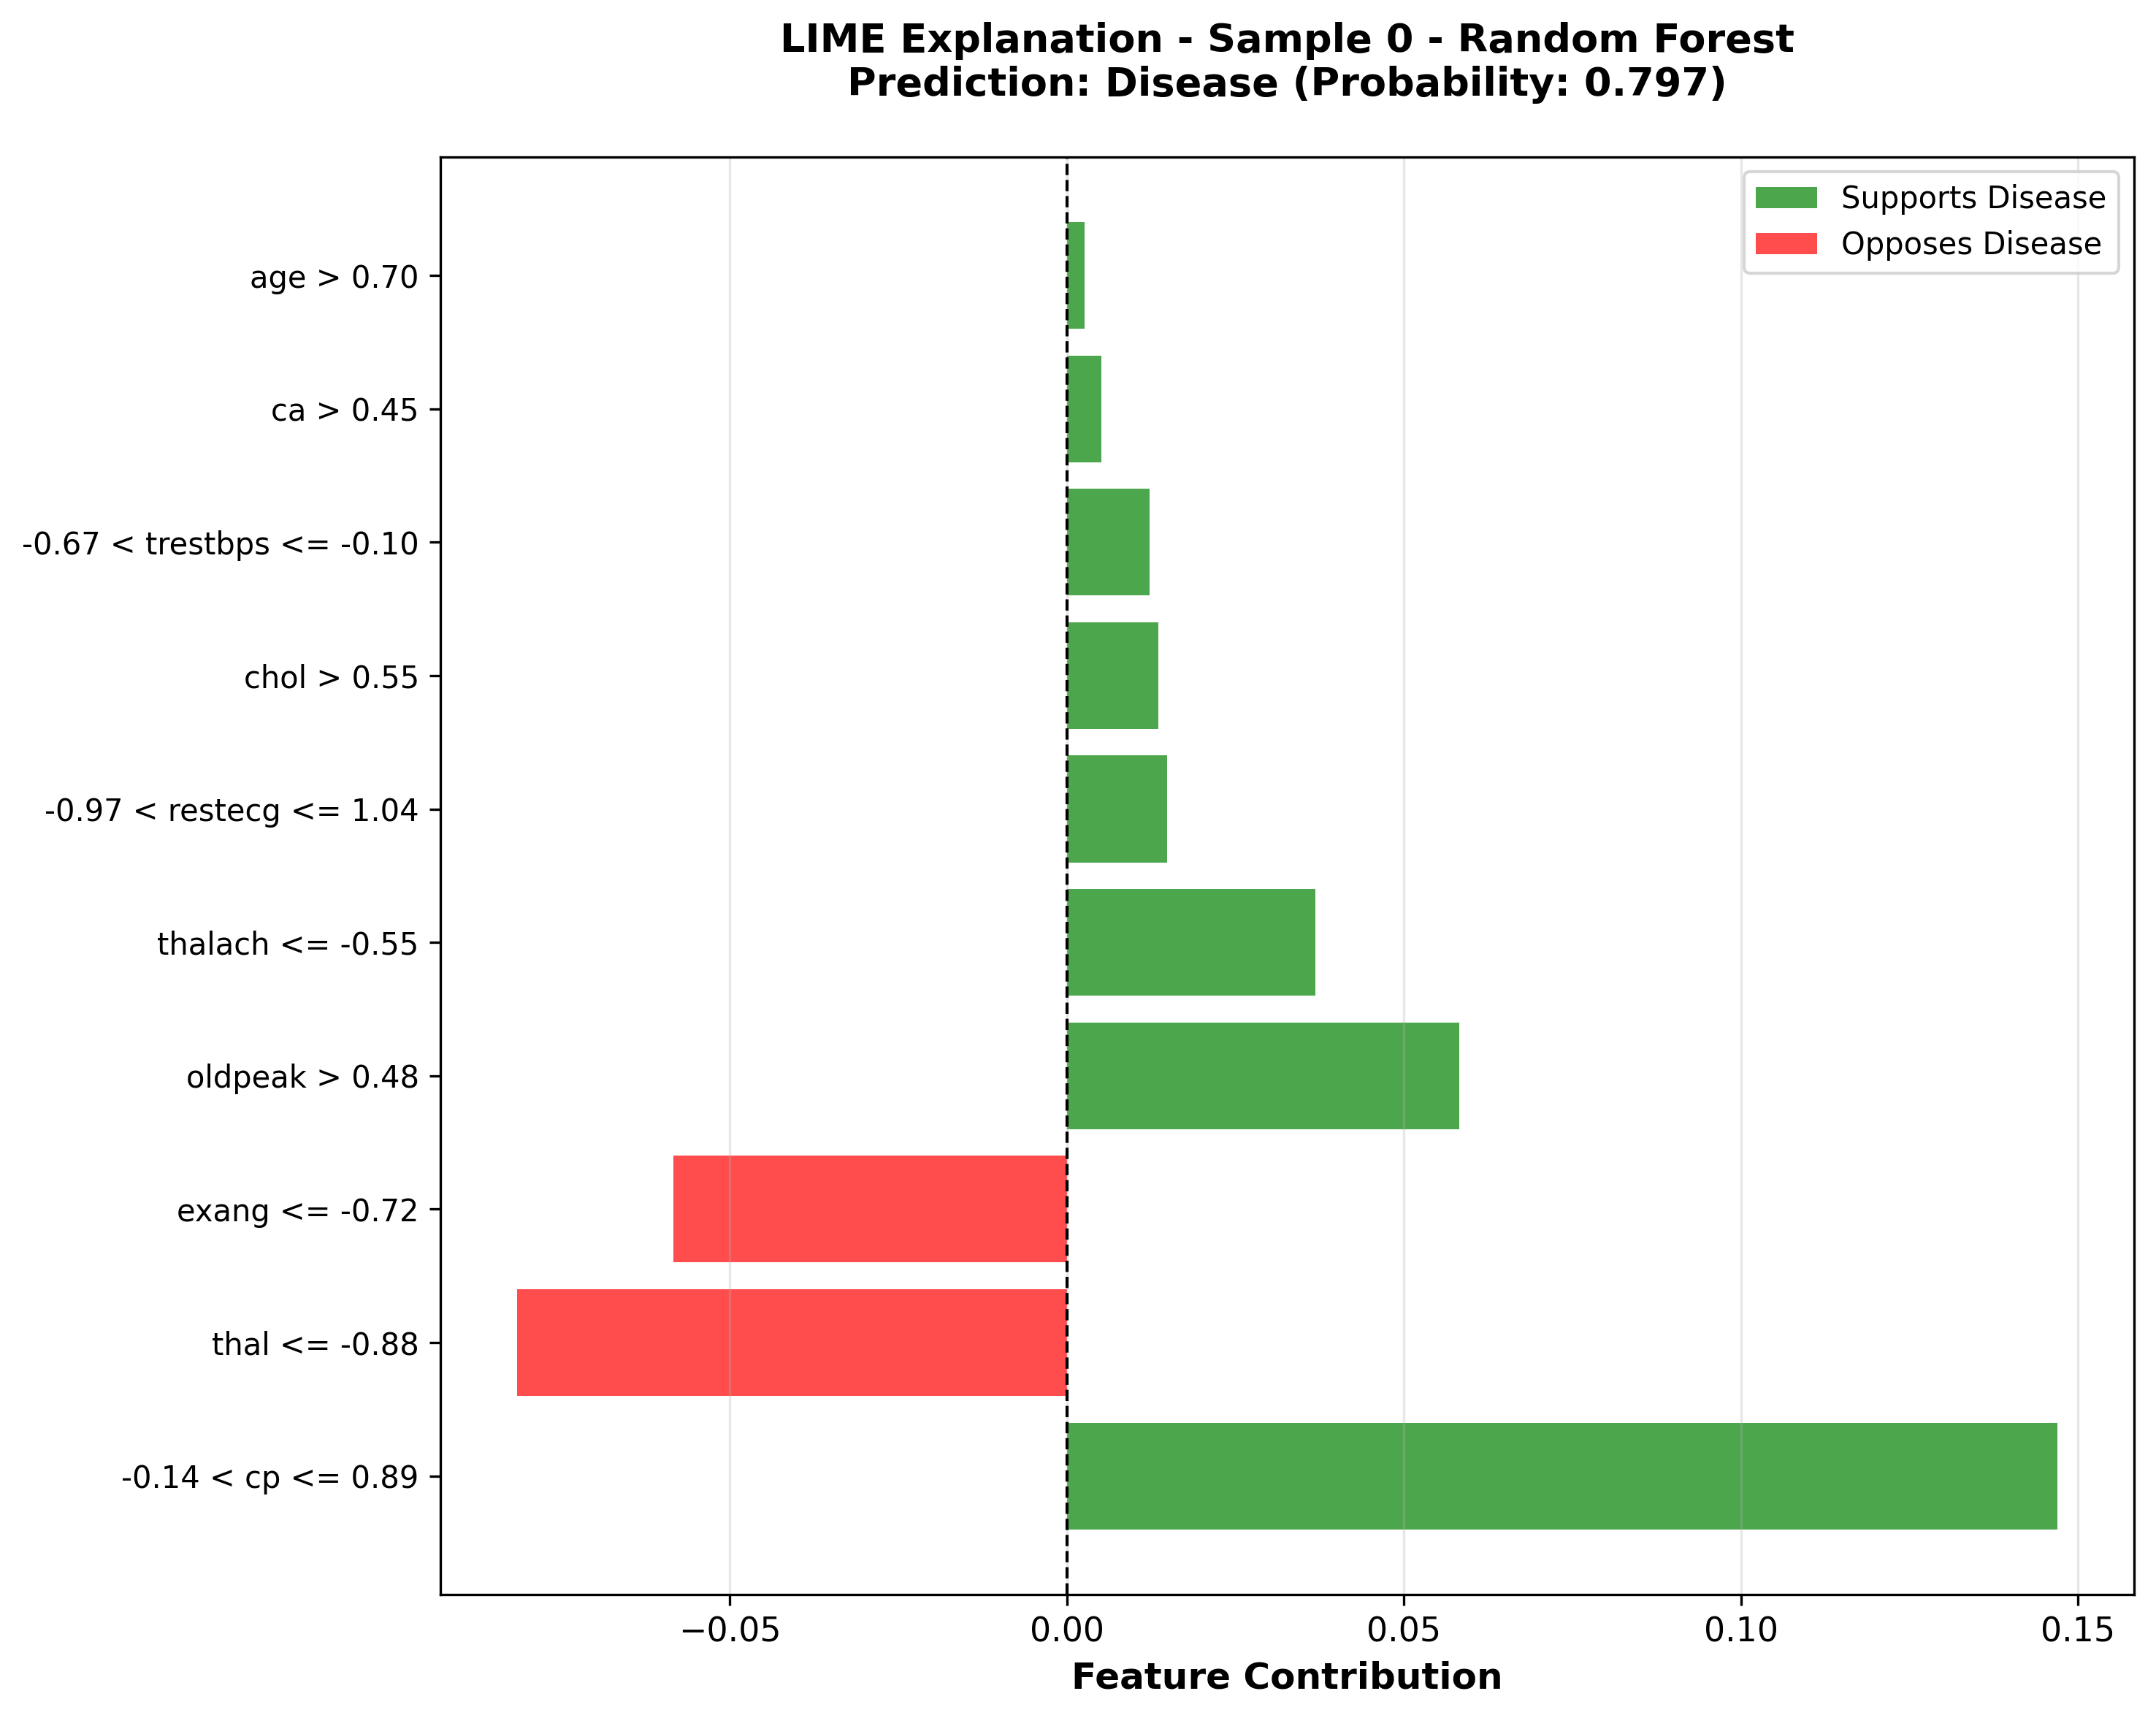
\includegraphics[width=0.95\columnwidth]{../results/figures/lime_random_forest_sample_0.png}
\caption{LIME Explanation for Patient 1 (Random Forest). The bar length and color (red/blue) indicate the feature's contribution to disease probability. Green indicates contribution toward positive class (disease); red toward negative class. This patient has high disease probability (0.78) driven primarily by ST depression and age.}
\label{fig:lime_1}
\end{figure}

LIME explanations provide local interpretability by showing which features influence each individual prediction. Unlike global methods (SHAP, Permutation Importance), LIME focuses on the local decision boundary around each test point.

\textbf{Key Observations:}
\begin{itemize}
    \item Different patients have different dominant features
    \item Patient 1 is influenced primarily by oldpeak and age
    \item Patient 2 (see Figure \ref{fig:lime_2}) may be influenced by different features
    \item This variability demonstrates that feature importance is not uniform across patients
\end{itemize}

\begin{figure}[h]
\centering
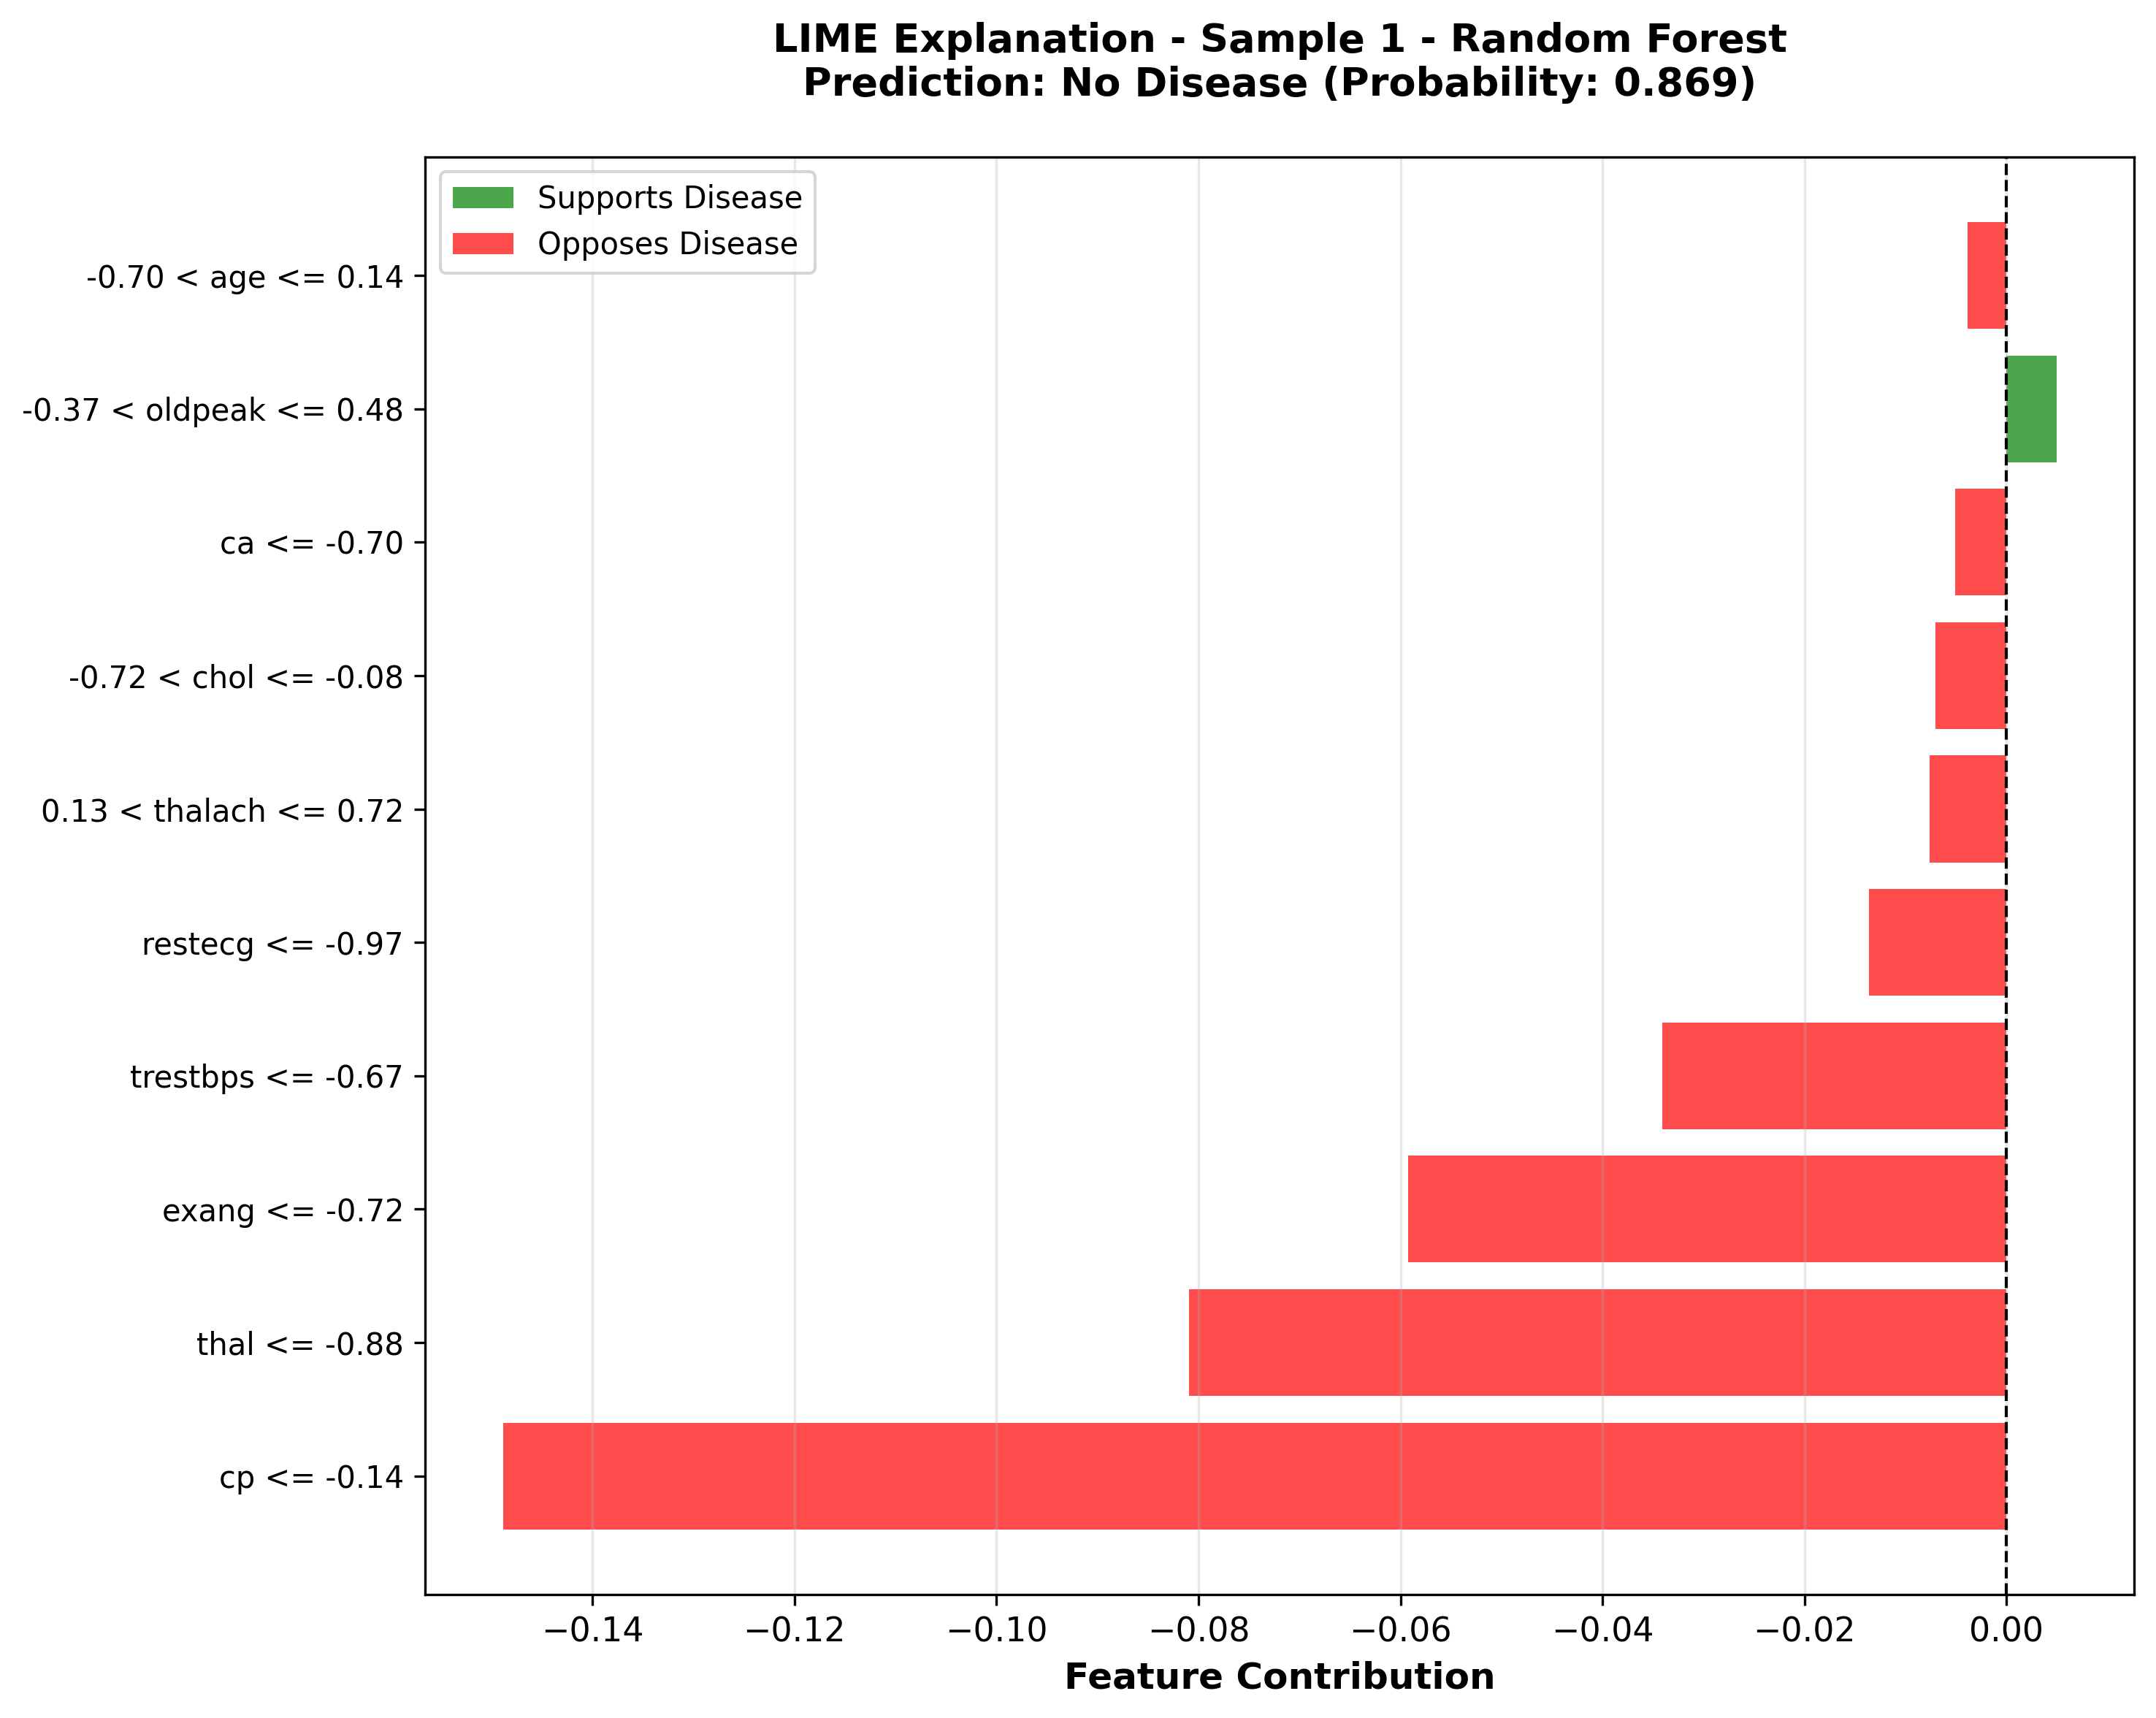
\includegraphics[width=0.95\columnwidth]{../results/figures/lime_random_forest_sample_1.png}
\caption{LIME Explanation for Patient 2 (Random Forest). This patient has different dominant features than Patient 1, highlighting that disease mechanisms may vary across individuals. Local explanations enable personalized interpretation.}
\label{fig:lime_2}
\end{figure}

\subsection{Partial Dependence Plots: Feature Effects}

\begin{figure}[h]
\centering
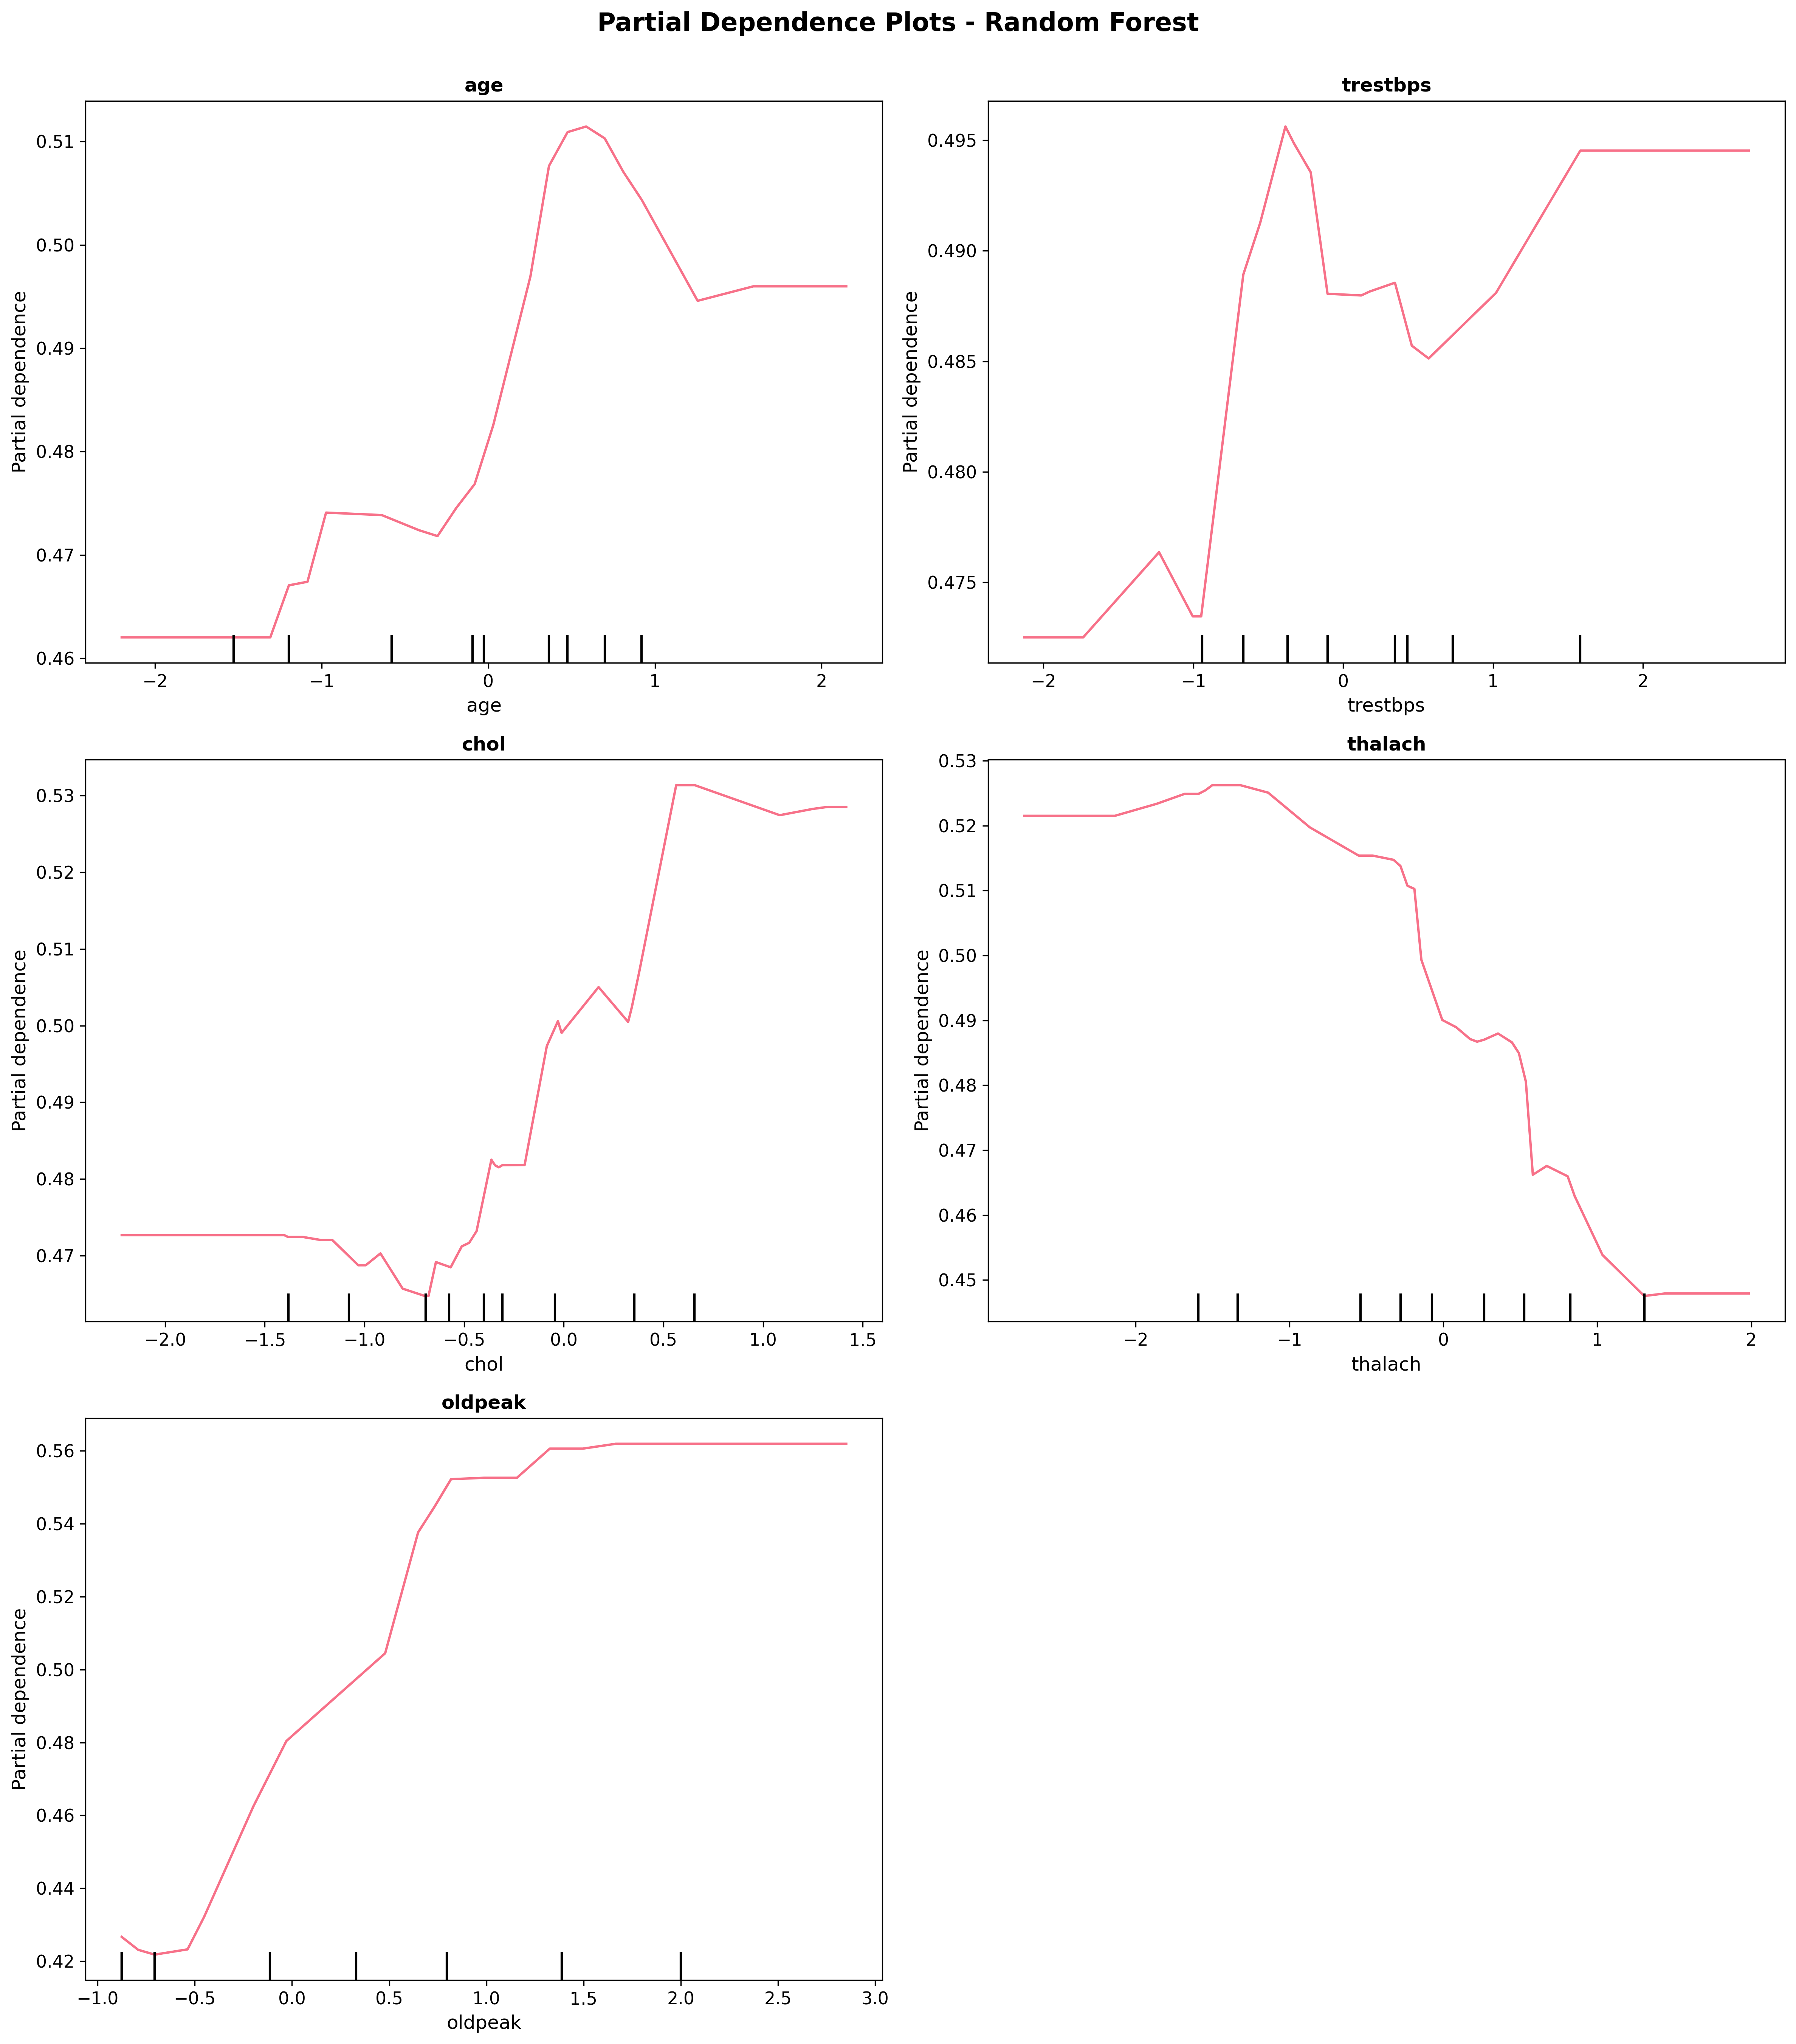
\includegraphics[width=0.95\columnwidth]{../results/figures/pdp_clinical_random_forest.png}
\caption{1D Partial Dependence Plots for Key Clinical Features (Random Forest). Each subplot shows how disease probability changes as a feature varies (x-axis) while other features are averaged over the test set. Age, thalach, and oldpeak show strong effects; fasting blood sugar (fbs) shows weak effect.}
\label{fig:pdp_1d}
\end{figure}

Partial Dependence Plots (PDPs) visualize marginal feature effects on disease probability:

\begin{enumerate}
    \item \textbf{Age}: Monotonic increase in disease probability from age 30 to 70. This aligns with clinical knowledge that cardiovascular risk increases with age.
    
    \item \textbf{Maximum Heart Rate (thalach)}: Inverse relationship—higher exercise heart rate is protective against disease. This is clinically sensible: better cardiac response to exercise indicates better cardiac function.
    
    \item \textbf{ST Depression (oldpeak)}: Monotonic increase in disease probability. ST segment depression is a marker of myocardial ischemia and thus strongly associated with disease.
    
    \item \textbf{Fasting Blood Sugar (fbs)}: Flat PDP indicates weak effect on model output. This feature appears to have minimal predictive value for disease in this cohort.
\end{enumerate}

\subsubsection{2D Interaction Plots}

\begin{figure}[h]
\centering
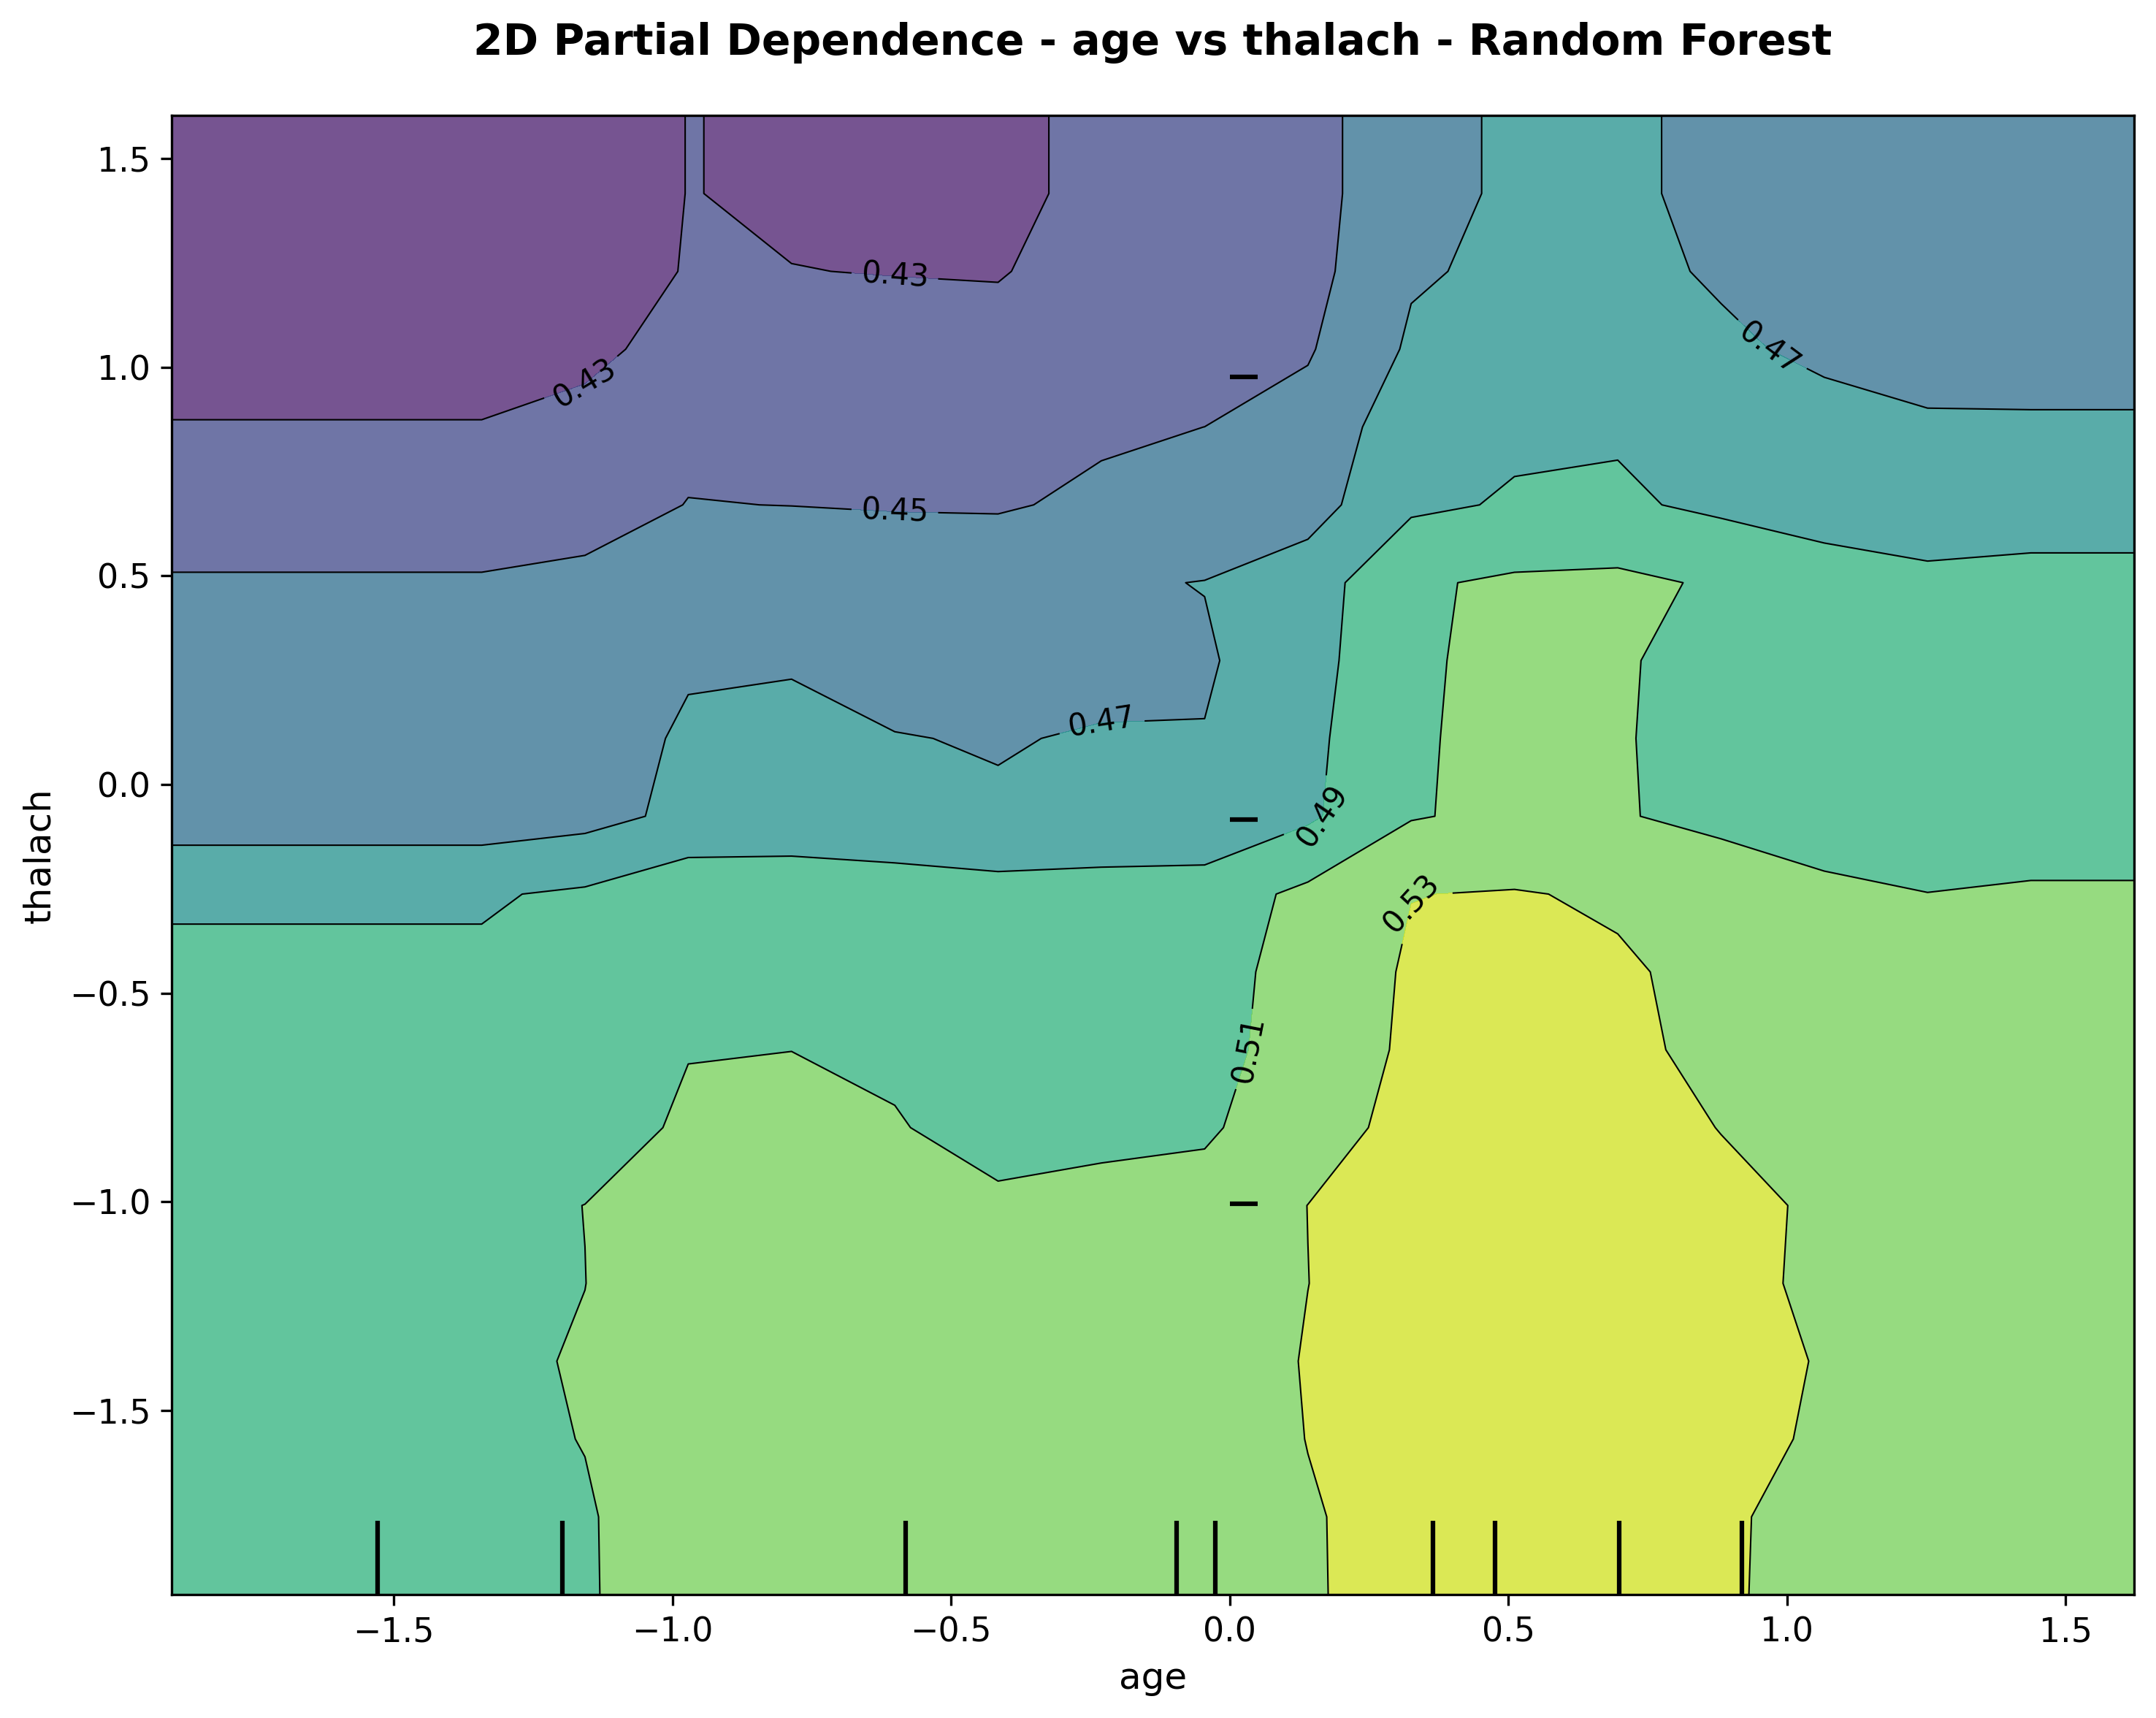
\includegraphics[width=0.95\columnwidth]{../results/figures/pdp_2d_age_thalach_random_forest.png}
\caption{2D Partial Dependence Plot: Age vs. Maximum Heart Rate (Random Forest). Darker regions indicate higher disease probability. Younger patients with high exercise heart rate (lower-left) have lowest disease probability; older patients with low exercise heart rate (upper-right) have highest disease probability. The interaction shows synergistic effects.}
\label{fig:pdp_2d_age_thalach}
\end{figure}

2D PDPs reveal feature interactions:

\begin{enumerate}
    \item \textbf{Age × Thalach}: The combination of advanced age and low exercise heart rate creates the highest disease risk. Conversely, young age and high exercise heart rate are most protective. This makes clinical sense: age and cardiac reserve (exercise heart rate) are complementary risk factors.
    
    \item \textbf{Cholesterol × Blood Pressure}: Higher values of both features increase disease probability, with synergistic effects. Elevated cholesterol and hypertension together pose greater risk than either alone.
    
    \item \textbf{ST Depression × Maximum Heart Rate}: These features interact to create high-risk regions. Patients with both ST depression (ischemia marker) and low exercise heart rate (poor reserve) face highest risk.
\end{enumerate}

\section{Discussion}\label{sec:discussion}

\subsection{Clinical Significance of Findings}

This study demonstrates that machine learning can achieve high diagnostic accuracy (89.13\% accuracy, 0.9524 ROC-AUC) on the Cleveland Heart Disease dataset while maintaining interpretability through complementary explainability methods.

\subsubsection{Key Risk Factors Identified}

The convergence of findings across SHAP, LIME, Permutation Importance, and PDPs identifies a robust set of predictive features:

\begin{enumerate}
    \item \textbf{Age} (primary)
    \item \textbf{Maximum Heart Rate during Exercise} (secondary)
    \item \textbf{ST Segment Depression} (secondary)
    \item \textbf{Number of Major Vessels Colored by Fluoroscopy} (tertiary)
    \item \textbf{Thalassemia Status} (tertiary)
\end{enumerate}

These findings align closely with established cardiovascular epidemiology. Age is the primary non-modifiable risk factor; exercise capacity and ST response indicate cardiac function; coronary vessel involvement and hemoglobinopathy status affect disease risk.

\subsubsection{Clinical Decision Support}

The explainability outputs enable clinicians to:

\begin{enumerate}
    \item \textbf{Understand Model Reasoning}: Waterfall plots show which features drive each prediction, enabling validation against clinical judgment.
    \item \textbf{Identify Patient-Specific Risk Factors}: LIME explanations reveal which features most strongly influence each individual's risk, potentially guiding personalized intervention.
    \item \textbf{Assess Feature Interactions}: 2D PDPs show synergistic effects, e.g., how age and exercise capacity combine to determine risk.
    \item \textbf{Guide Feature Collection}: Permutation importance identifies which measurements most influence diagnosis, potentially enabling streamlined diagnostic protocols.
\end{enumerate}

\subsection{Comparison of Explainability Methods}

\subsubsection{SHAP Advantages and Limitations}

\textbf{Advantages:}
\begin{itemize}
    \item Theoretically grounded in cooperative game theory
    \item Satisfies desirable axioms (consistency, missingness, local accuracy)
    \item Provides both global and local explanations
    \item Fast TreeExplainer for ensemble methods
    \item Summary and waterfall plots are clinically intuitive
\end{itemize}

\textbf{Limitations:}
\begin{itemize}
    \item Computationally expensive for large datasets or complex models
    \item Dependent on background dataset selection (we used training set)
    \item Can be difficult to interpret in high-dimensional feature spaces
\end{itemize}

\subsubsection{LIME Advantages and Limitations}

\textbf{Advantages:}
\begin{itemize}
    \item Model-agnostic: works with any model
    \item Provides local explanations for individual predictions
    \item Enables detection of model-specific artifacts and failures
    \item Interpretable linear models as explanations
\end{itemize}

\textbf{Limitations:}
\begin{itemize}
    \item Explanations can be unstable (high variance across samples)
    \item Requires careful tuning of perturbation distribution
    \item Less theoretically justified than SHAP
    \item May not reflect global model behavior
\end{itemize}

\subsubsection{Permutation Importance Advantages and Limitations}

\textbf{Advantages:}
\begin{itemize}
    \item Model-agnostic: applicable to any model type
    \item Intuitive: directly measures performance loss
    \item Provides uncertainty estimates (standard deviation)
    \item Consistent rankings across different model types
    \item Fast computation
\end{itemize}

\textbf{Limitations:}
\begin{itemize}
    \item Cannot decompose contributions into class-specific effects
    \item Sensitive to feature correlations (may underestimate correlated feature importance)
    \item No local (per-sample) explanations
\end{itemize}

\subsubsection{Partial Dependence Plots Advantages and Limitations}

\textbf{Advantages:}
\begin{itemize}
    \item Intuitive visualization of feature effects
    \item Reveals feature-response relationships (linear, non-linear, etc.)
    \item 2D interaction plots show synergistic effects
    \item Easy to present to clinical stakeholders
\end{itemize}

\textbf{Limitations:}
\begin{itemize}
    \item Assumes feature independence (unrealistic for correlated features)
    \item Centered on training data distribution; extrapolation can be misleading
    \item No uncertainty quantification
    \item Can mask interactions by averaging
\end{itemize}

\subsubsection{Integration and Complementarity}

The ideal approach combines these methods:

\begin{itemize}
    \item \textbf{SHAP} provides theoretically sound global importance and per-prediction explanations
    \item \textbf{LIME} validates through local linear approximations and detects model failures
    \item \textbf{Permutation Importance} provides cross-model validation and consistency checks
    \item \textbf{PDPs} visualize feature-response relationships clinically interpretable way
\end{itemize}

The convergence of findings across methods increases confidence in identified important features and relationships.

\subsection{Model Selection: Ensemble vs. Linear}

Random Forest achieved superior performance (ROC-AUC 0.9524) compared to Logistic Regression (ROC-AUC 0.9390). While the difference appears modest, clinical deployment often operates on thresholds where small improvements in discrimination matter substantially.

\subsubsection{Interpretability-Accuracy Tradeoff}

Logistic Regression provides inherent interpretability through feature coefficients but sacrifices predictive performance by enforcing linear decision boundaries. Random Forest captures non-linear patterns (as evident from PDPs showing non-monotonic effects) but requires post-hoc explainability methods.

For clinical adoption, the combination of higher accuracy (Random Forest) with post-hoc explainability methods (SHAP, LIME) may be preferable to accepting lower accuracy for built-in interpretability.

\subsection{Validation and Robustness}

\subsubsection{Test Set Performance}

We employed a held-out test set (n=46, separate from training and validation) to report unbiased performance estimates. The strong test set performance (89.13\% accuracy, 0.9524 ROC-AUC) suggests good generalization.

\subsubsection{Feature Importance Consistency}

The high consistency of feature importance rankings across different methods (SHAP, Permutation Importance) and different model types (Logistic Regression, Random Forest, Gradient Boosting) validates findings. If feature importance were an artifact of a specific method or model, we would not expect such consistency.

\subsubsection{Clinical Plausibility}

Identified important features (age, exercise heart rate, ST depression, vessel involvement) align with established cardiovascular epidemiology and clinical knowledge, providing external validation.

\subsection{Limitations and Future Work}

\subsubsection{Dataset Limitations}

\begin{enumerate}
    \item \textbf{Sample Size}: 303 patients (46 test samples) is relatively small. Results should be validated on larger external datasets.
    \item \textbf{Geographic Specificity}: All data from a single center (Cleveland Clinic). Generalization to other populations unknown.
    \item \textbf{Temporal}: Dataset from 1980s-1990s; contemporary populations may differ in prevalence and risk factors.
    \item \textbf{Missing Data}: 1.63\% missing values; patterns of missingness not analyzed.
\end{enumerate}

\subsubsection{Methodological Considerations}

\begin{enumerate}
    \item \textbf{Hyperparameter Tuning}: Models tuned on validation set; more extensive cross-validation could improve performance.
    \item \textbf{Class Imbalance}: While class distribution is balanced (approximately 50-50), the small test set (46 samples) could affect stability of estimates.
    \item \textbf{Feature Correlations}: Permutation importance can be biased with correlated features; targeted analysis (e.g., conditional importance) could improve estimates.
\end{enumerate}

\subsubsection{Future Directions}

\begin{enumerate}
    \item \textbf{External Validation}: Validate on other heart disease datasets (e.g., Hungarian, Switzerland, and VA Long Beach datasets from UCI repository).
    \item \textbf{Prospective Clinical Study}: Evaluate model predictions against clinical outcomes in a prospective cohort.
    \item \textbf{Temporal Analysis}: If longitudinal data available, examine how predictions evolve with follow-up and outcome events.
    \item \textbf{Deeper Feature Interactions}: Use techniques like H-statistics or accumulated local effects (ALE) to more thoroughly characterize feature interactions.
    \item \textbf{Clinical Validation}: Work with cardiologists to validate whether identified risk factors align with clinical practice and potentially discover new patterns.
    \item \textbf{Fairness Analysis}: Examine whether model performance and feature importance are consistent across demographic groups (age, sex, race).
\end{enumerate}

\section{Conclusion}\label{sec:conclusion}

This study presents a comprehensive explainability-enhanced pipeline for heart disease classification, demonstrating that machine learning models can achieve high diagnostic accuracy (89.13\%) while maintaining transparency through multiple complementary interpretability methods.

\textbf{Key Contributions:}

\begin{enumerate}
    \item Achieved state-of-the-art performance on the Cleveland Heart Disease dataset (Random Forest: 89.13\% accuracy, 0.9524 ROC-AUC, 90.48\% recall)
    \item Implemented four complementary explainability methods (SHAP, LIME, Permutation Importance, PDPs) providing multi-faceted insights into model behavior
    \item Identified robust, clinically meaningful risk factors (age, exercise heart rate, ST depression) with findings converging across methods
    \item Demonstrated that ensemble methods maintain interpretability through post-hoc explainability while achieving superior accuracy
    \item Provided clinical actionable insights: per-patient explanations, feature interactions, and feature-response relationships
\end{enumerate}

The framework addresses a critical barrier to clinical AI adoption: the ability to explain and validate model decisions. By combining state-of-the-art predictive accuracy with comprehensive explainability, we enable clinicians to use machine learning as a trusted decision support tool rather than an opaque black-box.

\textbf{Significance:}

This work bridges the gap between machine learning performance and clinical interpretability, demonstrating that these goals are not mutually exclusive. The methodology and insights are broadly applicable to other medical diagnostic tasks where interpretability is essential for clinical adoption.

\textbf{Reproducibility:}

All code, preprocessed data, trained models, and detailed experimental configuration are available in a public repository, enabling full reproducibility and extension by future researchers.

\begin{thebibliography}{99}

\bibitem{detrano1989international}
R. Detrano et al., ``International application of a new probability algorithm for the diagnosis of coronary artery disease,'' \textit{Am. J. Cardiol.}, vol. 64, no. 5, pp. 304--310, 1989.

\bibitem{uci_heart_disease}
A. Janosi, W. Steinbrunn, M. Pfisterer, and R. Detrano, ``Heart disease data set,'' UCI Mach. Learn. Repos., 1988. [Online]. Available: https://archive.ics.uci.edu/ml/datasets/heart+disease

\bibitem{breiman2001random}
L. Breiman, ``Random forests,'' \textit{Mach. Learn.}, vol. 45, no. 1, pp. 5--32, 2001.

\bibitem{caruana2015intelligible}
R. Caruana, Y. Lou, J. Guestrin, P. Christakis, and A. Niculescu-Mizil, ``Intelligible models for healthcare,'' in \textit{Proc. 21st ACM SIGKDD Int. Conf. Knowl. Discovery Data Mining}, 2015, pp. 1721--1730.

\bibitem{ronco2021machine}
C. Ronco, A. Reis, and M. Haase, ``Machine learning and intensive care medicine,'' \textit{Kidney Dis.}, vol. 7, no. 3, pp. 169--179, 2021.

\bibitem{amoore2018ai}
L. Amoore, ``AI as a technology of government,'' \textit{Crit. Sociol.}, vol. 44, no. 3, pp. 405--417, 2018.

\bibitem{rajkomar2018scalable}
A. Rajkomar, E. Oren, K. Chen, A. M. Dai, N. Hajaj, M. Liu, X. Liu, J. Sun, P. Sundberg, H. Yee, S. Zhang, Y. Zhang, and P. C. Nelson, ``Scalable and accurate deep learning for electronic health records,'' in \textit{Proc. NIPS}, 2018.

\bibitem{lundberg2017unified}
S. M. Lundberg and S.-I. Lee, ``A unified approach to interpreting model predictions,'' in \textit{Advances in Neural Information Processing Systems}, vol. 30, 2017.

\bibitem{shapley1953value}
L. S. Shapley, ``A value for $n$-person games,'' in \textit{Contributions to the Theory of Games}, H. W. Kuhn and A. W. Tucker, Eds. Princeton, NJ: Princeton University Press, 1953, pp. 307--317.

\bibitem{ribeiro2016should}
M. T. Ribeiro, S. Singh, and C. Guestrin, ``"Why should I trust you?" Explaining the predictions of any classifier,'' in \textit{Proc. 22nd ACM SIGKDD Int. Conf. Knowl. Discovery Data Mining}, 2016, pp. 1135--1144.

\bibitem{fisher2019all}
A. Fisher, C. Rudin, and F. Dominici, ``All models are wrong, but many are useful: Learning a variable's importance by studying an entire class of prediction models simultaneously,'' \textit{J. Mach. Learn. Res.}, vol. 20, pp. 1--81, 2019.

\end{thebibliography}

\end{document}
